% allgem. Dokumentenformat
\documentclass[a4paper,12pt,headsepline]{scrartcl}
%Variablen welche innerhalb der gesamten Arbeit zur Verfügung stehen sollen
\newcommand{\titleDocument}{Bachelor Thesis}
\newcommand{\subjectDocument}{in Computer Science}


\newcommand{\specialcell}[2][c]{%
	\begin{tabular}[#1]{c}
		#2
	\end{tabular}
}

\newcommand{\specialcellleft}[2][@{}l]{%
	\begin{tabular}[#1]{@{}l}
		#2
	\end{tabular}
}

\newcommand{\fixme}[1]{
	~\\
	\noindent
	\textbf{\textcolor{red}{FIXME: #1}}
	\\
}




% weitere Pakete
% Grafiken aus PNG Dateien einbinden
\usepackage{graphicx}

% Eurozeichen einbinden
\usepackage[right]{eurosym}

\usepackage{ctable}

% Umlaute unter UTF8 nutzen
\usepackage[utf8]{inputenc}

% Zeichenencoding
\usepackage[T1]{fontenc}

\usepackage{lmodern}
\usepackage{fix-cm}

\usepackage{svg}

% floatende Bilder ermöglichen
%\usepackage{floatflt}

% mehrseitige Tabellen ermöglichen
\usepackage{longtable}

% Unterstützung für Schriftarten
%\newcommand{\changefont}[3]{ 
%\fontfamily{#1} \fontseries{#2} \fontshape{#3} \selectfont}

\setcounter{secnumdepth}{4}
\setcounter{tocdepth}{4}

% Packet für Seitenrandabständex und Einstellung für Seitenränder
\usepackage{geometry}
\geometry{left=3.5cm, right=2cm, top=2.5cm, bottom=2cm}

% Paket für Boxen im Text
\usepackage{fancybox}

% bricht lange URLs "schoen" um
\usepackage[hyphens,obeyspaces,spaces]{url}

% Paket für Textfarben
\usepackage{color}

% Mathematische Symbole importieren
\usepackage{amssymb}

% auf jeder Seite eine Überschrift (alt, zentriert)
%\pagestyle{headings}

% erzeugt Inhaltsverzeichnis mit Querverweisen zu den Kapiteln (PDF Version)
\usepackage[bookmarksnumbered,pdftitle={\titleDocument},hyperfootnotes=false]{hyperref} 
%\hypersetup{colorlinks, citecolor=red, linkcolor=blue, urlcolor=black}
%\hypersetup{colorlinks, citecolor=black, linkcolor= black, urlcolor=black}

% neue Kopfzeilen mit fancypaket
\usepackage{fancyhdr} %Paket laden
\pagestyle{fancy} %eigener Seitenstil
\fancyhf{} %alle Kopf- und Fußzeilenfelder bereinigen
\fancyhead[L]{\nouppercase{\leftmark}} %Kopfzeile links
\fancyhead[C]{} %zentrierte Kopfzeile
\fancyhead[R]{\thepage} %Kopfzeile rechts
\renewcommand{\headrulewidth}{0.4pt} %obere Trennlinie
%\fancyfoot[C]{\thepage} %Seitennummer
%\renewcommand{\footrulewidth}{0.4pt} %untere Trennlinie

% für Tabellen
\usepackage{array}

% Runde Klammern für Zitate
%\usepackage[numbers,round]{natbib}

% Festlegung Art der Zitierung - Havardmethode: Abkuerzung Autor + Jahr
\bibliographystyle{alphadin}

% Schaltet den zusätzlichen Zwischenraum ab, den LaTeX normalerweise nach einem Satzzeichen einfügt.
\frenchspacing

% Paket für Zeilenabstand
\usepackage{setspace}

% für Bildbezeichner
\usepackage{capt-of}

% für Stichwortverzeichnis
\usepackage{makeidx}

% für Listings
\usepackage{listings}
\lstset{numbers=left, numberstyle=\tiny, numbersep=5pt, keywordstyle=\color{black}\bfseries, stringstyle=\ttfamily,showstringspaces=false,basicstyle=\footnotesize,captionpos=b}
\lstset{language=java}

% Indexerstellung
\makeindex

% Abkürzungsverzeichnis
\usepackage[english]{nomencl}
\let\abbrev\nomenclature

% Abkürzungsverzeichnis LiveTex Version
\renewcommand{\nomname}{Abbreviations}
\setlength{\nomlabelwidth}{.25\hsize}
\renewcommand{\nomlabel}[1]{#1 \dotfill}
\setlength{\nomitemsep}{-\parsep}
\makenomenclature
%\makeglossary

% Abkürzungsverzeichnis TeTEX Version
% \usepackage[german]{nomencl}
% \makenomenclature
% %\makeglossary
% \renewcommand{\nomname}{Abkürzungsverzeichnis}
% \setlength{\nomlabelwidth}{.25\hsize}
% \renewcommand{\nomlabel}[1]{#1 \dotfill}
% \setlength{\nomitemsep}{-\parsep}

% Disable single lines at the start of a paragraph (Schusterjungen)
\clubpenalty = 10000
% Disable single lines at the end of a paragraph (Hurenkinder)
\widowpenalty = 10000
\displaywidowpenalty = 10000

\begin{document}
% hier werden die Trennvorschläge inkludiert
%hier müssen alle Wörter rein, welche Latex von sich auch nicht korrekt trennt bzw. bei denen man die genaue Trennung vorgeben möchte
\hyphenation{
Film-pro-du-zen-ten
Lux-em-burg
Soft-ware-bau-steins
zeit-in-ten-siv
}

%Schriftart Helvetica
%\changefont{phv}{m}{n}

% Leere Seite am Anfang
\newpage
\thispagestyle{empty} % erzeugt Seite ohne Kopf- / Fusszeile

% Titelseite %
% das Papierformat zuerst
%\documentclass[a4paper, 11pt]{article}

% deutsche Silbentrennung
%\usepackage[ngerman]{babel}

% wegen deutschen Umlauten
%\usepackage[ansinew]{inputenc}

% hier beginnt das Dokument
%\begin{document}


\thispagestyle{empty}

%\begin{figure}[t]
% \includegraphics[width=0.6\textwidth]{abb/fh_koeln_logo}
%\end{figure}

\begin{figure}[t]
 \centering
 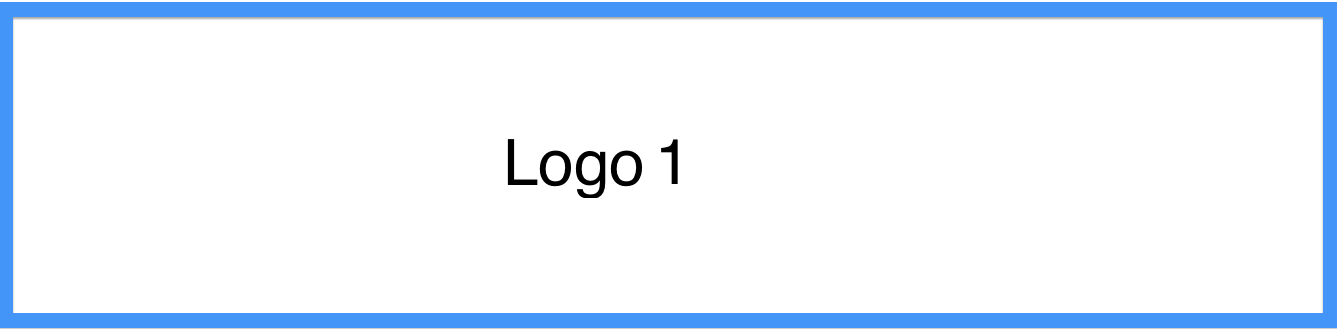
\includegraphics[width=0.6\textwidth]{abb/logo1}
~~~~~~~~~~
 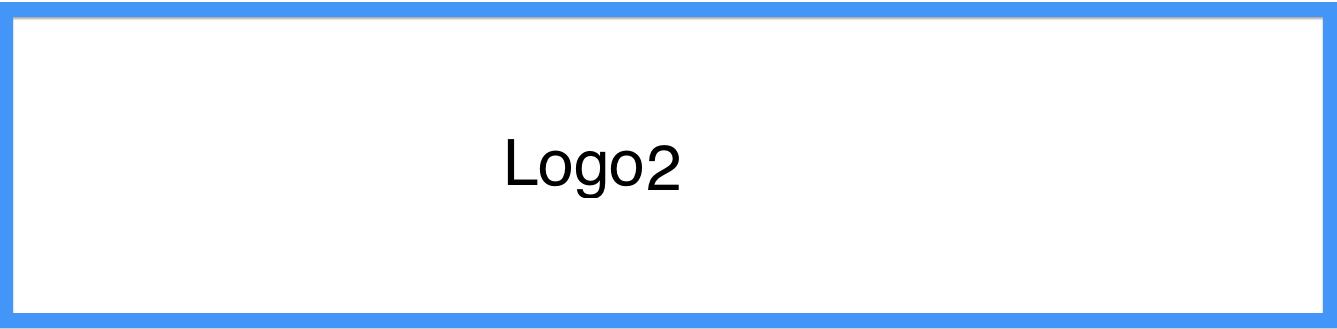
\includegraphics[width=0.20\textwidth]{abb/logo2}
\end{figure}


\begin{verbatim}


\end{verbatim}

\begin{center}
\Large{University of Bayreuth}\\
\end{center}


\begin{center}
\Large{Institute for Computer Science}
\end{center}
\begin{verbatim}








\end{verbatim}
\begin{center}
\doublespacing
\textbf{\LARGE{\titleDocument}}\\
\singlespacing
\begin{verbatim}

\end{verbatim}
\textbf{{~\subjectDocument}}
\end{center}
\begin{verbatim}

\end{verbatim}
\begin{center}

\end{center}
\begin{verbatim}






\end{verbatim}
\begin{flushleft}
\begin{tabular}{llll}
\textbf{Topic:} & & Integration of JPA-conform ORM-Implementations & \\
	& & in Hibernate Search & \\
& & \\
\textbf{Author:} & & Martin Braun <martinbraun123@aol.com>& \\
& & Matrikel-Nr. 1249080 & \\
& & \\
\textbf{Version date:} & & \today &\\
& & \\
\textbf{1. Supervisor:} & & Prof. Dr. Stefan Jablonski &\\
\textbf{2. Supervisor:} & & Prof. Dr. Bernhard Westfechtel &\\
\end{tabular}
\end{flushleft}
%
%\pagebreak
%~
%\pagebreak

%\begin{verbatim}






















%\end{verbatim}

%\begin{center}
%	To my parents.
%\end{center}

%\afterpage{\null\newpage}
%\pagebreak
%~\\\\
%\pagebreak
%~

% römische Numerierung
%\pagenumbering{arabic}

% 1.5 facher Zeilenabstand
\onehalfspacing

% Einleitung / Abstract
% !TeX spellcheck = en_GB
\section*{Abstract}

Fulltext search engines are a powerful tool to improve query results in applications where relational databases don't suffice. However, they don't integrate well with the widely spread concept of object relationship mappers (ORM, in Java predominantly represented by the standard JPA) in the object oriented programming world.
\\\\
This is where Hibernate Search comes into use for Java developers: It combines JPA and fulltext search by being the intermediary between Hibernate ORM and a Lucene based fulltext index. It has one problem though: Hibernate Search only works with Hibernate ORM but not with other JPA-conform providers even though it is possible to support these. In this thesis we will show how such a generic version can be accomplished.
\\\\
After discussing the methods we use, we give an explanation why a generic Hibernate Search is a desirable solution for JPA developers. Creating it is challenging as we have to build a standalone version of Hibernate Search's internal engine first and then integrate it with JPA together with an automatic index updating mechanism. We solve these challenges and give a usage example of the completed generic version. Finally, we discuss the current development state of the generic version and give an outlook on the planned merging process with the original Hibernate Search.

\pagebreak

\section*{Zusammenfassung}
Volltextsuchengines sind ein wertvolles Werkzeug um Suchergebnisse in Anwendungen zu verbessern, wenn relationale Datenbanken nicht ausreichen. Diese Engines sind jedoch nicht gut mit dem in der objekt-orientierten Programmierungs-Welt weit verbreiteten Konzept der Objekt-Relationalen Mapper (ORM, in Java vor allem durch den Standard JPA repräsentiert) integriert. 
\\\\
Für Java Entwickler bietet hier Hibernate Search eine Abhilfe: Es kombiniert JPA und Volltextsuche und stellt die Schnittstelle zwischen Hibernate ORM und einem Lucene basierten Volltextindex dar. Es hat aber ein Problem: Hibernate Search funktioniert nur in Kombination mit Hibernate ORM, aber nicht mit anderen JPA konformen Providern, obwohl es möglich wäre diese zu unterstützen. In dieser Thesis wird daher gezeigt, wie eine solche generische Version realisiert werden kann.
\\\\
Nachdem die benutzten Methoden erklärt wurden, wird eine Begründung dafür gegeben, warum Hibernate Search eine wünschenswerte Lösung für JPA Entwickler ist. Diese zu entwickeln ist eine Herausforderung, da wir zuerst eine Standalone Version von Hibernate Search's interner Engine bauen müssen, um diese danach in eine JPA Version zusammen mit einem automatischen Index Updating Mechanismus zu integrieren. Wir zeigen wie diese Probleme gelöst werden und erklären die Benutzung anhand eines Beispiels. Zuletzt gehen wir auf den aktuellen Entwicklungsstand der generischen Version ein und geben einen Ausblick auf den geplanten Merge-Prozess mit dem originalen Hibernate Search.



% einfacher Zeilenabstand
\singlespacing

% Inhaltsverzeichnis anzeigen
\newpage
~
\newpage
\tableofcontents
~
\pagebreak

% das Abbildungsverzeichnis
%\newpage
% Abbildungsverzeichnis soll im Inhaltsverzeichnis auftauchen
%\addcontentsline{toc}{section}{List of figures}
% Abbildungsverzeichnis endgueltig anzeigen
%\listoffigures

% das Tabellenverzeichnis
%\newpage
% Abbildungsverzeichnis soll im Inhaltsverzeichnis auftauchen
%\addcontentsline{toc}{section}{Tabellenverzeichnis}
% \fancyhead[L]{Abbildungsverzeichnis / Abkürzungsverzeichnis} %Kopfzeile links
% Abbildungsverzeichnis endgueltig anzeigen
%\listoftables

%% WORKAROUND für Listings
%\makeatletter% --> De-TeX-FAQ
%\renewcommand*{\lstlistoflistings}{%
%  \begingroup
%    \if@twocolumn
%      \@restonecoltrue\onecolumn
%    \else
%      \@restonecolfalse
%    \fi
%    \lol@heading
%    \setlength{\parskip}{\z@}%
%    \setlength{\parindent}{\z@}%
%    \setlength{\parfillskip}{\z@ \@plus 1fil}%
%    \@starttoc{lol}%
%    \if@restonecol\twocolumn\fi
%  \endgroup
%}
%\makeatother% --> \makeatletter
% das Listingverzeichnis
%\newpage
% Listingverzeichnis soll im Inhaltsverzeichnis auftauchen
%\addcontentsline{toc}{section}{Listingverzeichnis}
%\fancyhead[L]{Abbildungs- / Tabellen- / Listingverzeichnis} %Kopfzeile links
%\renewcommand{\lstlistlistingname}{Listingverzeichnis}
%\lstlistoflistings
%%%%

% das Abkürzungsverzeichnis
%\newpage
% Abkürzungsverzeichnis soll im Inhaltsverzeichnis auftauchen
%\addcontentsline{toc}{section}{Abkürzungsverzeichnis}
% das Abkürzungsverzeichnis entgültige Ausgeben
%\fancyhead[L]{Abkürzungsverzeichnis} %Kopfzeile links
%\nomenclature{UGC}{User Generated Content}
\nomenclature{CSS}{Cascading Style Sheets}
\nomenclature{JS}{JavaScript}
\nomenclature{SQL}{Structured Query Language}
\nomenclature{GPL}{GNU General Public License}
\nomenclature{GNU}{GNU is not Unix}
\nomenclature{LGPL}{GNU Lesser General Public License}
\nomenclature{XMPP}{Extensible Messaging and Presence Protocol}
\nomenclature{IM}{Instant Message}
\nomenclature{CMS}{Content Management System}
\nomenclature{RSS}{Really Simple Syndication}
\nomenclature{JSON}{JavaScript Object Notation}
\nomenclature{HTML}{Hypertext Markup Language}
\nomenclature{TDD}{Test-driven development}
\nomenclature{GUI}{Graphical User Interface}
\nomenclature{KPI}{Key Performance Indicator}
\nomenclature{WWW}{World Wide Web}
\nomenclature{OCR}{Optical Character Recognition}
\nomenclature{ERM}{Entity Relationship Modell}

%\printnomenclature

% Definiert Stegbreite bei zweispaltigem Layout
\setlength{\columnsep}{25pt}

%%%%%%% EINLEITUNG %%%%%%%%%%%%
%\twocolumn
\newpage
\fancyhead[L]{\nouppercase{\leftmark}} %Kopfzeile links

% 1,5 facher Zeilenabstand
\onehalfspacing

% einzelne Kapitel
% !TeX spellcheck = en_GB

\section{Preface}\label{Preface}
In the software world, or more specific, the Java enterprise world, developers tend to abstract access to data in a way that components are interchangeable. A perfect example for such an abstraction is the usage of Object Relational Mappers (ORM). The database specifics are mostly uninteresting to the average developer and the need for native SQL is brought down to a minimum. This makes the switch to a different relational database system (RDBMS) easier in the later stages of a product's life cycle.
\\\\
The Java Persistence API (JPA) went even further by providing a standard for ORMs. First conceived in 2006 as part of EJB 3.0 \footnote{JSR 220: Enterprise Java Beans 3.0, see~\cite{jsr_jpa1}} \footnote{Javaworld: Understanding JPA, Part 1, see~\cite{javaworld_jpa1}}, it is now the de-facto standard for Object Relational Mappers in Java. The developer doesn't need to know which specific ORM is used in the application, as all the database queries are written against a standardized query API and are therefore portable. This means that not only the database is interchangeable, but even the specific ORM, it is accessed by, is as well.
\\\\
However, this does not mean that all JPA implementations come with the same features. While all of them are JPA compliant (apart from minor bugs), some ship with additional modules to enhance their capabilities. A perfect example for this is the Hibernate Search API aimed at Hibernate ORM users.\footnote{Hibernate ORM project homepage, see~\cite{hibernate_orm}} \footnote{Hibernate Search project homepage, see~\cite{hibernate_search_homepage}}
\\\\

\pagebreak
\noindent
Nowadays, even small applications like online shops need enhanced search capabilities to let the user find more results for a given input.
This is not something a regular RDBMS excels at and Hibernate Search comes into use as shown in figure \ref{fig1}: It works atop the Hibernate ORM, a popular JPA implementation, and enables the developer to index the domain model for searching. It's not only a mapper from JPA entities to a search index, but also keeps the index up-to-date if something in the database changes.
\\
\begin{figure}[ht]
	\centering
	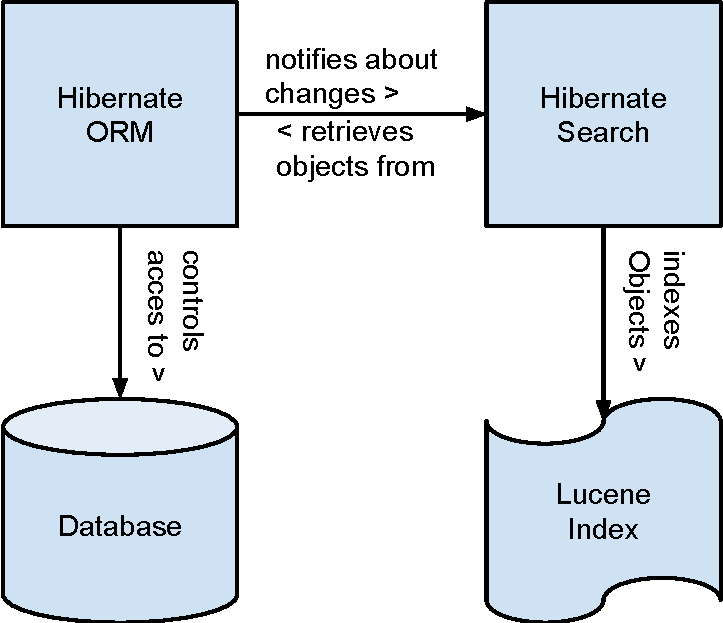
\includegraphics[scale=0.45]{images/hibernate_search_hibernate_schema.pdf}
	\caption{Hibernate Search with Hibernate ORM}
	\label{fig1}
\end{figure}
\\
Hibernate Search is based on the powerful Lucene search toolbox \footnote{sourcecode on Hibernate Search GitHub, see~\cite{hsearch_source_code_git}} \footnote{Hibernate Search FAQ, see~\cite{hibernate_search_faq}} and is a separate project in the Hibernate family and aims to provide a JPA "feeling" in its API as it also incorporates a lot of JPA interfaces in its codebase. However, this does not mean that it is compatible with other JPA providers than Hibernate ORM (apart from Hibernate OGM, the NoSQL JPA mapper of the family) as the following figure \ref{fig2} shows.
\\\\
\begin{figure}[ht]
	\centering
	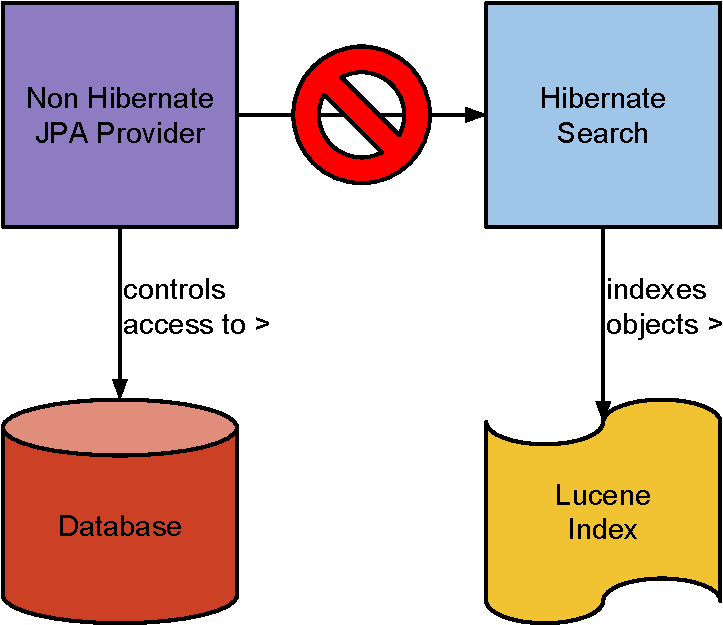
\includegraphics[scale=0.45]{images/hibernate_search_any_jpa_problem_schema.pdf}
	\caption{Hibernate Search's incompatibility with other JPA implementations}
	\label{fig2}
\end{figure}
\\
While using Hibernate Search obviously is beneficial for Hibernate ORM applications, not all developers can bind themselves to a specific JPA implementation in their application. For some, the ability to change implementations might be of strategic importance, for others it could just be sheer preference to use a different JPA implementation.

\noindent
Currently, developers that do not want to bind themselves to Hibernate ORM have to resort to using different full text search systems like native Lucene\footnote{official Lucene website, see~\cite{lucene_apache_org}}, ElasticSearch\footnote{ElasticSearch Java API, see~\cite{elasticsearch_java_api}} or Solr\footnote{Solr Java API, see~\cite{solr_java_api}}. While this is always a viable option, for some applications Hibernate Search would be a much better suit because of its design with a entity structure in mind and the automatic index updating feature, if it just were compatible with generic JPA.
\\\\
When investigating Hibernate Search's project structure
\footnote{Hibernate Search GitHub repository, see~\cite{hsearch_source_code_git}}, we can see that the only module apart from some server-integration modules that depends on any ORM logic is "hibernate-search-orm". The modules that contain the indexing engine, the replication logic, alternative backends, etc. are completely independent from any ORM logic. This means, that most of the codebase could be reused for a generic version of Hibernate Search.
\\\\
\noindent
Creating such a generic Hibernate Search is a better approach for a search API on top of JPA rather than rewriting a JPA binding from scratch. Hibernate Search could then act as an all-purpose API for fulltext search in the JPA world instead of having a competing API that would just do the same thing in a different style.
\\
\begin{figure}[ht]
	\centering
	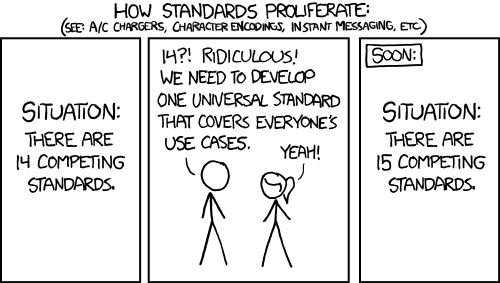
\includegraphics[scale=0.5]{images/competing_standards.png}
	\caption{xkcd.com on competing standards \protect\footnotemark}
	\label{xkcd_standards_fig}
\end{figure}
\footnotetext{xkcd comic \#927, see~\cite{xkcd_competing_standards_source}}
\\
This is why we will show how such a generic version can be built in this thesis. First, we will look at how Hibernate Search's engine can be reused. Then, we will write a standalone version of this engine and finally integrate it with generic JPA.

\pagebreak

\noindent
\textbf{Short overview of contents}:
\\\\
\noindent
In chapter \ref{Methods} we explain what methods we are using to build Hibernate Search GenericJPA. In chapter \ref{Overview} we give an overview over the relevant technologies used in this thesis and give short introductions to several fulltext search engines and the reasoning behind Hibernate Search GenericJPA. In chapter \ref{Challenges} we introduce a small example project and explain the main challenges while developing Hibernate Search GenericJPA. In chapter \ref{standalone_chapter} we describe a standalone version of Hibernate Search. In chapter \ref{integration_jpa} we explain how the JPA integration of the standalone version is designed. In chapter \ref{automatic_indexing_chapter} we work out an automatic index updating mechanism for Hibernate Search GenericJPA. In chapter \ref{usage_chapter} we give a full explanation of how to use Hibernate Search GenericJPA using the example from chapter \ref{Challenges}. In chapter \ref{outlook} we give a summary of we have achieved in this thesis and describe further steps.

\pagebreak

\pagebreak

\section{Methods} \label{Methods}

While developing the generic version of Hibernate Search we are using the following process schema to find the solutions for the all the different problems:

\begin{figure}[ht]
	\centering
	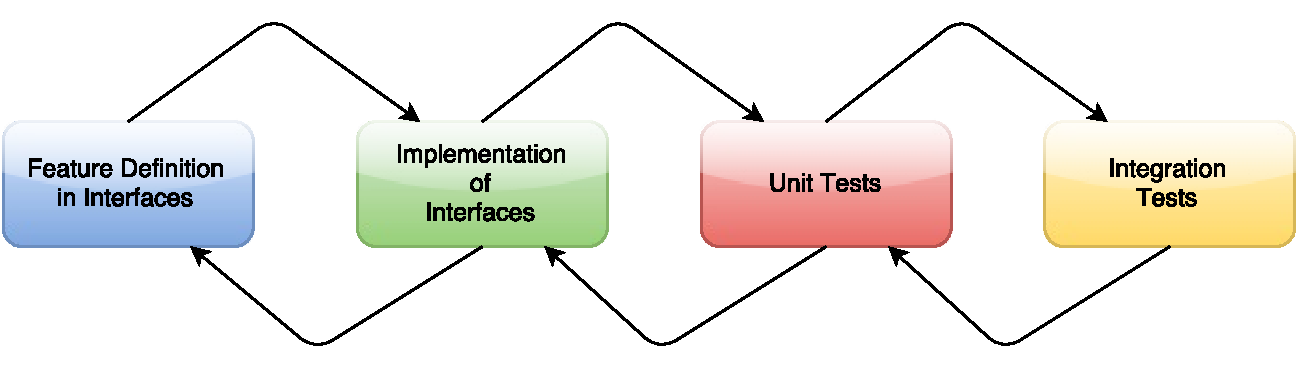
\includegraphics[scale=0.52]{images/work_process.pdf}
	\caption{Development Process}
	\label{development_process_of_a_feature}
\end{figure}

\begin{itemize}
	\item \textbf{Requirements Engineering}: As part of the solution finding process for each problem, we start by specifying a requirements specification that consists of:
	\begin{itemize}
		\item "a specification of the context in which the system will operate,
		\item a list of desired system functions of the system,
		\item a definition of the semantics of these functions,
		\item and a list of quality attributes of those functions" \footnote{Web Engineering, chapter: Requirements Engineering: Problem Analysis and Solution Specification, R. J. Wieringa, 2004, see~\cite{requirements_engineering}}
	\end{itemize}
	While 
	\item \textbf{Feature Definition in Interfaces}: As the next step, the requirements are translated into Java interfaces.	While modelling the interfaces we try to be as compliant to the \textbf{Single Responsibility Principle} \footnote{objectmentor.com: Article on Single Responsibility Principle, see~\cite{singleresponsibility_objectmentor}} as possible because it enforces structures that are easy to reuse and change due to being pluggable single purpose classes. However we explicitly break it in some cases to allow more user-friendly interfaces (mostly in API entry-points).
	\\
	By defining the features in interfaces and using them instead of implementations to write code, we achieve complete independence between the implementing classes and are compliant to the \textbf{Open-Closed-Principle} \footnote{	objectmentor.com: Article on Open-Closed-Principle, see~\cite{openclosed_objectmentor}} internally ("Modules should be both open (for extension) and closed (for modification)" \footnote{Object-Oriented Software Construction, Prentice Hall, 1988, Bertrand Meyer, see~\cite{openclosed_bertrand}}) which allows us to write more "pluggable" code.
	\item \textbf{Implement Interfaces}: Once the interfaces are properly defined, we write implementations for these according to the contracts set. These classes generally don't use other implementations directly and build functionality only by using interfaces.
	\item \textbf{Unit Test}: Each feature has to have a corresponding unit test. These are necessary to test each implementation for the right behaviour (outputs and side-effects) for at least one given input. They also help to identify bugs in the implementations.
	\item \textbf{Integration Test}: While Unit-Tests check the behaviour of every \textit{single} feature implementation, integration tests are used to cover the correct behaviour when used together with the other parts of the project. With these tests we ensure all features interoperate properly with each other.
\end{itemize}
\noindent
Note that once a step is finished, that doesn't mean it is final. As we can see in the diagram, we can go back and forth between the different steps at will to adapt to specific implementation problems and new problems that have not been covered before.
\\\\
We choose this kind of on-the-fly structure because it suits the project best: We have to investigate different approaches before we can work out the real solution, first. Additionally, because "hibernate-search-engine" is an internal API, we have to be as flexible as possible with our development since some features of it can be different than what we might expect in the first place.
\\\\
It is worth mentioning that all the tests (including the integration tests) are executed during each build to ensure no regression bugs occur. This is automatically managed by the Maven \footnote{Maven project homepage, see~\cite{maven_homepage}} build tool.
\\\\
This process is embedded in a combined approach of \textbf{top-down} \footnote{Top-down programming, Robert Strandh, see~\cite{top_down_strandh}} and \textbf{bottom-up} \footnote{Bottom-up programming, Robert Strandh, see~\cite{bottom_up_strandh}} to software development: After dividing the project into submodules (top-down) we develop the building blocks first and integrate them into bigger mechanisms (the sub-modules) as the project goes on (bottom-up). This way we stay flexible in the early stages of development and only have to write "wiring code" in the later stages.

\pagebreak


% !TeX spellcheck = en_GB

\section{Overview of technologies}\label{Overview}
Before we can go into detail about how to work with Hibernate Search in a generic environment, we will give a short overview of the relevant technologies first. We will explain why ORMs in general and the JPA specification in particular are beneficial. Then, we will explain what fulltext search engines are used for and give a short overview about the available solutions for Java. We will see that generalizing Hibernate Search for any JPA implementation is a good approach and that it has benefits over using the different search solutions available.

\subsection{Object Relational Mappers}
Nowadays, many popular languages like Java, C\#, etc. are object oriented\footnote{Wikipedia on Object Oriented Programming (OOP), see~\cite{object_oriented_programming_wiki}}.
While SQL solutions for querying relational databases exist for these languages (JDBC for Java\footnote{Oracle JDBC overview, see~\cite{jdbc_oracle}}, OleDb for C\#\footnote{OleDb usage page, see~\cite{oledb_ms}}), the user either has to work with the rowsets manually or convert them into custom data transfer objects (DTO) to gain at least some "real" objects to work with. Both approaches don't suit the object oriented paradigm well as SQL "flattens" the data into rows when querying while a well designed class model would work with multiple classes in a hierarchy.
\\
\lstset{language=sql}
\begin{lstlisting}[frame=htrbl, caption={SQL "flattening" the author and book table into rows}, label={lst:flattening.sql}]
SELECT author.id, author.name, book.id, book.name 
FROM author_book, author, book
WHERE author_book.bookid = book.id
AND author_book.authorid = author.id
\end{lstlisting}
~\\
This is one of the points where Object Relational Mappers (ORM) come into use. They map tables to entity-classes and
enable users to write queries against these classes instead of tables. The returned objects are part of a complex object hierarchy and are easier to use from a object oriented point of view.
\\
\lstset{language=java}
\begin{lstlisting}[frame=htrbl, caption={ORM query example}, label={lst:flattening.sql}]
List<Author> data = orm.query("SELECT a FROM Author a");
for(Author author : data) {
	// we can still fetch the books without joining in the query
	System.out.println("name: " + author.getName() + 
		", books: " + author.getBooks());
}
\end{lstlisting}
\noindent
This is especially useful if used in big software products as not all programmers have to know the exact details of the underlying database. The database system could even be completely replaced by another (provided the ORM supports the specific RDBMS), while the business logic would not change a bit.

\subsection{JPA}

The first version of the JPA standard was released in May 2006. From then on it rose to being probably the most commonly used persistence API for Java and is considered the "industry standard approach for Object Relational Mapping"\footnote{Wikibooks on Java Persistence, see~\cite{wikibooks_on_jpa}}. While mostly known for standardizing relational database mappers (ORM), it also supports other concepts like NoSQL\footnote{Hibernate OGM project homepage, see~\cite{hibernate_ogm}} \footnote{EclipseLink project homepage, see~\cite{eclipselink}} or XML storage\footnote{EclipseLink project homepage, see~\cite{eclipselink}}. However, when talking about JPA in this thesis, we will be focusing on the relational aspects of it. Currently, the newest version of this standard is 2.1 \footnote{JSR 338: JPA 2.1 specification, see~\cite{jpa_21_jcp}} \footnote{Wikipedia on Java Persistence API, see~\cite{wiki_jpa}}.
\\\\
Some popular relational implementations are:
\begin{itemize}
	\item Hibernate ORM (Red Hat)\footnote{Hibernate ORM project homepage, see~\cite{hibernate_orm}}
	\item EclipseLink (Eclipse foundation)\footnote{EclipseLink project homepage, see~\cite{eclipselink}}
	\item OpenJPA (Apache foundation)\footnote{OpenJPA project homepage, see~\cite{openjpa}}
\end{itemize}
~\\
Using the standardized JPA API over any native ORM API has one really interesting benefit:
The specific JPA implementation can be swapped out as it comes with standards for many common use cases.
\\\\
This is particularily important if you are working in a Java EE environment. Java EE itself is a specification for platforms, mostly Web-servers (JPA is part of the Java EE spec).\footnote{Wikipedia on Java EE, see~\cite{wiki_java_ee}} Many Java EE Web-servers ship with a bundled JPA implementation that they are optimized for (Wildfly with Hibernate ORM, GlassFish with EclipseLink, ...). This means that if the server is switched, it could also be a reasonable idea to swap out the JPA implementor. If everything in the application is written in a JPA compliant way, the user will then generally not run into many problems related to this switch.

\pagebreak

\subsection{Fulltext search engines}

Conventional relational databases are good at retrieving and querying structured data. But if one wants to build a search engine atop a domain model, most RDBMS will only support the SQL-LIKE operator \footnote{w3schools on SQL LIKE, see~\cite{sql_like_w3schools}}:\\

\lstset{language=sql}
\begin{lstlisting}[frame=htrbl, caption={SQL LIKE operator in use}, label={lst:result2}]
SELECT book.id, book.name FROM book WHERE book.name LIKE %name%;
\end{lstlisting}
While this might be enough for some applications, this wildcard query doesn't support features a good search engine would need, for example:

\begin{itemize}
	\item fuzzy queries (variations of the original string will get matched, too)
	\item phrase queries (search for a specified phrase)
	\item regular expression queries (matches are determined by a regular expression)
	\item stemming and language specific optimisations
	\item comprehensive synonym support
\end{itemize}
There may exist some RDBMS that support similar query-types, but in the context of using an ORM we would then lose the ability to switch databases since we would use vendor-specific features not every RDBMS supports.
\\\\
Fulltext search engines can be used to complement databases in this regard. They are generally not intended to be replacing the database, but add additional functionality by indexing the data that is to be searched in a more sophisticated way. We will now take a look at some of the most popular available options for Java developers (including Hibernate Search) focusing on their usage and features. After that we will give the reasoning behind why a \textbf{generic} Hibernate Search is preferable to the other solutions.

\pagebreak

\subsubsection{Lucene}

\begin{quote}
	Apache Lucene™ is a high-performance, full-featured text search engine library written entirely in Java. It is a technology suitable for nearly any application that requires full-text search, especially cross-platform.\footnote{official Lucene website, see~\cite{lucene_apache_org}}
\end{quote}
Lucene serves as the basis for many fulltext search engines written in Java. It has many different utilities and modules aimed at search engine developers. However, it can be used on its own as well. Its latest stable version is 5.3.0 \footnote{official Lucene website, see~\cite{lucene_apache_org}}.

\paragraph{Concepts}

As Lucene's focus is not on storing relational data, it comes with its own set of concepts. Following is a short overview over the most important ones. These are not only the basis for Lucene, but also for the other search engines we will discuss next, as they are based on Lucene's rich set of features.

\subparagraph{Index structure}
Lucene uses an \textbf{inverted index} to store data. This means that instead of storing texts mapped to the words contained in them, it works the other way around. All different words (terms) are mapped to the texts they occur in\footnote{Lucene basic concepts, see~\cite{lucene_basic_concepts}}, so it can be compared to a \(Map<String, List<Text>>\) in Java. Before anything can be searched using Lucene, it has to be added to the the index (indexed) first.

\subparagraph{Documents}
Documents are the data-structure Lucene stores and retrieves from the index. An index can contain zero or more Documents.

\subparagraph{Fields}
A Document consists of at least one field. Fields are basically tuples of key and value. They can be stored (retrievable from the index) and/or indexed (used for searches, generate hits).

\subparagraph{Analyzers}
Before documents get indexed, their fields are analysed with one of the many Analyzers first. Analysis is the process of modifying the input in a manner such that it can be searched upon (stemming, tokenization, ...).

\pagebreak

\subparagraph{Example index}
The following figure \ref{inverted_index} shows how an inverted index schematically looks like in Lucene. On the left we can see three different documents containing an id and the two text fields "field1" and "field2". The inverted index that stores references to these documents can be seen on the right. It contains all the different terms (field \& value) mapped to the id of the texts they are contained in. The values of these terms have been analysed before they were stored into the index as they only contain singular words instead of the original "sentences" from the left.
\\
\begin{figure}[ht]
	\centering
	\begin{minipage}{0.4\textwidth} 
		\centering
		\begin{tabular}{|c|c|c|}
			\hline
			\multicolumn{3}{|c|}{Documents} \\
			\specialrule{.2em}{0em}{0em}
			id & field1 & field2 \\
			\specialrule{.1em}{0em}{0em}
			1 & \specialcell{fulltext search \\ lucene} & search \\
			\hline
			2 & lucene search & java \\
			\hline
			3 & fulltext java & fulltext lucene \\
			\hline
		\end{tabular}
	\end{minipage}
	% Auffüllen des Zwischenraums
	\hfill
	\begin{minipage}{0.4\textwidth}
		\centering
		\begin{tabular}{|c|c|c|}
			\hline
			\multicolumn{3}{|c|}{Inverted Index} \\
			\specialrule{.2em}{0em}{0em}
			\multicolumn{2}{|c|}{Term} & Occurences \\
			\hline
			Field & Value & \\
			\specialrule{.1em}{0em}{0em}
			field1 & fulltext & 1,3 \\
			\hline
			field1 & search & 1,2 \\
			\hline
			field1 & lucene & 1,2 \\
			\hline
			field1 & java & 3 \\
			\hline
			field2 & search & 1 \\
			\hline
			field2 & java & 2 \\
			\hline
			field2 & fulltext & 3 \\
			\hline
			field2 & lucene & 3 \\
			\hline
		\end{tabular}
	\end{minipage}
	\caption{schematic inverted index}
	\label{inverted_index}
\end{figure}

\pagebreak

\paragraph{Usage}
Using Lucene as a standalone engine requires the programmer to design the engine from the bottom up. The developer has to write all the logic, starting with the actual indexing code through to the code managing access to the index. The conversion from Java objects to Documents (for indexing) and back (for searching) have to be implemented as well. This whole process requires a lot of code to be written and the API only helps by providing the necessary tools. This has one additional problem: The Lucene API tends to change a lot between versions and the code has to be kept up-to-date. It's not uncommon that whole features that were state-of-the-art in one version, are deprecated (potentially unstable, marked to be removed in the future) in the next release, resulting in big code changes being potentially necessary.

\paragraph{Features}
Lucene probably is the most complete toolbox to build a search-engine from. It has pre-built analyzers for many languages, a queryparser to support generating queries out of user input, a phonetic module, a faceting module, and many other features. While mostly known for its fulltext capabilities, it also has modules used for other purposes, for example the spatial module that enables geo-location query support.
\\\\
One benefit of its low-level API is that it can easily be extended with custom analyzers, query-types, etc, though. This is especially useful for more sophisticated search engines.

\pagebreak

\subsubsection{Fulltext search servers: ElasticSearch and Solr}
Lucene is the basis for two of the most popular Lucene based search servers available: ElasticSearch (by elastic)\footnote{ElasticSearch Homepage, see~\cite{elasticsearch_homepage}} and Solr (sister project of Lucene)\footnote{Solr Homepage, see~\cite{solr_homepage}}. Their current stable versions are 1.7.1 \footnote{ElasticSearch Download website, see~\cite{elasticsearch_downloads_website}} and 5.3.0 \footnote{Solr Homepage, see~\cite{solr_homepage}} respectively.

\paragraph{Usage}
As both ElasticSearch and Solr are standalone server applications, they have to be configured before they can be used similar to the process of setting up a RDBMS. As they don't ship with any authentication mechanism by default they also have to be secured before they are used in production \footnote{Solr security, see~\cite{solr_security}} \footnote{elastic Shield (security for ElasticSearch), see~\cite{elasticsearch_security}}. Index changes and queries are done via a REST-like API (among other options).

\paragraph{Features}
As ElasticSearch and Solr are built upon Lucene, they support the same basic features that Lucene does, but add additional indexing and searching functionality and come with their own stack of tools to ease their usage (index inspectors, load analyzers, ... \footnote{Solr Administration (Core Specific Tools), see~\cite{solr_admin}} \footnote{ElasticHQ, see~\cite{elasticsearch_admin}}). They are generally used because of their good clustering capabilities (distribution \& replication) and are optimized for high throughput and scalability \footnote{ElasticSearch: Life inside a cluster, see~\cite{elasticsearch_clustering}} \footnote{Solr: Introduction to Scaling and Distribution, see~\cite{solr_clustering}}. As they are not running inside the client application (as a native Lucene implementation would) these kind of servers don't force the user to use a specific programming language (in our case a JVM based one like Java).

\pagebreak

\subsubsection{Hibernate Search}

From the GitHub README of Hibernate Search:
\begin{quote}
Full text search engines like Apache Lucene are very powerful technologies to add efficient free text search capabilities to applications. However, Lucene suffers several mismatches when dealing with object domain models. Amongst other things indexes have to be kept up to date and mismatches between index structure and domain model as well as query mismatches have to be avoided.

Hibernate Search addresses these shortcomings - it indexes your domain model with the help of a few annotations, takes care of database/index synchronization and brings back regular [JPA] managed objects from free text queries. \footnote{Hibernate Search GitHub README, see~\cite{hsearch_source_code_git}}
\end{quote}
\noindent
Hibernate Search's current stable version is 5.3.0.Final which is based on Lucene 4.10.4 \footnote{hibernate-search-engine on mvnrepository.org, see~\cite{hibernate_search_engine_mvnrepository}}.

\paragraph{Usage}
Hibernate Search is used in the context of JPA compliant applications using Hibernate ORM. It can easily be used by adding it to the classpath and setting some configuration properties in the JPA persistence.xml and integrates with JPA interfaces seamlessly. 

\paragraph{Features}
Similar to ElasticSearch and Solr Hibernate Search is built upon Lucene and has similar features regarding indexing, searching and clustering but it is designed to be used in a JPA environment: it indexes JPA entities and the queries return them again.
\\\\
It is tightly coupled with Hibernate ORM: while an integration with JPA is existent, Hibernate Search doesn't allow other JPA implementations than Hibernate ORM to be used as it internally relies on its code.
\\\\
For future versions the Hibernate Search team is planning on adding ElasticSearch and Solr as additional backends besides the already existing Lucene based backend and the optional Infinispan integration.

\pagebreak

\subsubsection{Why a generic Hibernate Search?}

For Hibernate ORM developers Hibernate Search is probably currently the easiest way to have fulltext search capabilities in their application. While the native Lucene backend might not be the perfect choice for some applications (because they want to share the index with applications written in e.g. C\#), the planned ElasticSearch and Solr backends would make up for this in the future.
\\\\
Developers using other JPA implementations like EclipseLink or OpenJPA currently don't have the option to use a similar API to Hibernate Search as the Compass project has been discontinued (last version: 2.2.0 from Apr 06, 2009 as of mvnrepository.org \footnote{see \url{http://mvnrepository.com/artifact/org.compass-project/compass/2.2.0}}).
\\\\
In order to create a fulltext engine integrated with generic JPA creating a separate solution similar to Hibernate Search wouldn't be beneficial as it would include a lot of work and would probably not get much recognition.
\\\\
A generic version of Hibernate Search however would use (most of) the already existing interfaces and would require a lot less code for the same behaviour and features as nearly all of the important Lucene logic can be found in modules not having any notion of Hibernate ORM. In fact, the only module of Hibernate Search requiring Hibernate ORM is "hibernate-search-orm".
\\\\
Ultimately this generic version of Hibernate Search could also be used to inspire remodelling of the original Hibernate Search to incorporate generic JPA, which would probably make Hibernate Search the de-facto standard for fulltext search for the complete JPA world.
\\\\
Using Hibernate Search and turning it into a general standard is definitely better than writing everything from scratch and thus "reinventing the wheel". \label{reinvent_the_wheel}

\pagebreak

% !TeX spellcheck = en_GB
\section{Challenges}\label{Challenges}
While building the generic version of Hibernate Search, we will encounter some challenges. We will now discuss the biggest ones and introduce a small example project. This project will be used to showcase some problems and usages later on in this thesis as well.

\subsection{The example project} \label{example_project}
Consider a software built with JPA that is used to manage the inventory of a bookstore. It stores information about the available books (ISBN, title, genre, short summary of the contents) and the corresponding authors (surrogate id, first \& last name, country) in a relational database. Each author is related to zero or more Books and each Book is written by one or more Authors. The entity relationship model diagram defining the database looks like this:
\\
\begin{figure}[ht]
	\centering
	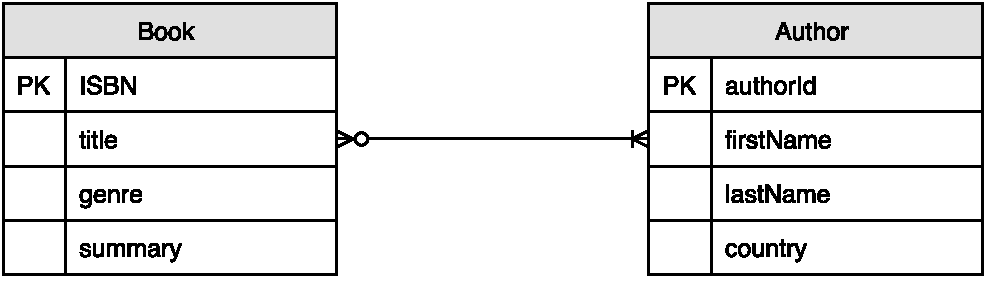
\includegraphics[scale = 0.9]{images/Sample_Project_ER.pdf}
	\caption{the bookstore entity relationship model}
	\label{fig3}
\end{figure}
\\
Using a mapping table for the M:N relationship of Author and Book, the database contains three tables: Author, Book and Author\_Book. The JPA annotated classes for these entities are defined as following:
\\
\lstset{language=java}
\begin{lstlisting}[frame=htrbl, caption={Book.java}, label={lst:book.java_1}]
@Entity
@Table(name = "Book")
public class Book {

	@Id
	@Column(name = "isbn")
	private String isbn;
	
	@Column(name = "title")
	private String title;
	
	@Column(name = "genre")
	private String genre;
	
	@Lob
	@Column(name = "summary")
	private String summary;
	
	@ManyToMany(mappedBy = "books", cascade = {
		CascadeType.MERGE,
		CascadeType.DETACH,
		CascadeType.PERSIST,
		CascadeType.REFRESH
	})
	private Set<Author> authors;
	
	//getters & setters ...
}
\end{lstlisting}

\lstset{language=java}
\begin{lstlisting}[frame=htrbl, caption={Author.java}, label={lst:author.java_1}]
@Entity
@Table(name = "Author")
public class Author {
	
	@Id
	@GeneratedValue(strategy = GenerationType.AUTO)
	@Column(name = "authorId")
	private Long authorId;
	
	@Column(name = "firstName")
	private String firstName;
	
	@Column(name = "lastName")
	private String lastName;
	
	@Column(name = "country")
	private String country;
	
	@ManyToMany(cascade = {
		CascadeType.MERGE, 
		CascadeType.DETACH, 
		CascadeType.PERSIST, 
		CascadeType.REFRESH
	})
	@JoinTable(name = "Author_Book", 
		joinColumns = 
			@JoinColumn(name = "authorFk", 
				referencedColumnName = "authorId"),
		inverseJoinColumns = 
			@JoinColumn(name = "bookFk", 
				referencedColumnName = "isbn"))
	private Set<Book> books;
	
	//getters & setters ...
}
\end{lstlisting}
For the sake of simplicity and since every JPA provider is able to derive a default DDL script from the annotations, we don't supply any information about how to create the schema here. However, for real world applications defining a hand-written DDL script might be a better idea since the generated code might not be optimal and differs between the different JPA implementations and RBDMSs used.

\subsection{Indexing \& searching} \label{problem_indexing_searching}
Hibernate Search's engine wasn't designed to be used directly by application developers. Its main purpose is to serve as an integration point for other APIs that need to leverage its power to index object graphs and query the index for hits. This is why we have to write our own standalone module based on the "hibernate-search-engine" to ease its general usage. After the standalone is finished, we will build an integration of it with JPA to mimic the usage of Hibernate Search ORM as good as possible. By incorporating the same engine that the original does, we keep almost all of the indexing behaviour and even stay compatible with entities designed for it.

\subsection{Index rebuilding}
If the way objects are indexed changes, the existing files have to be purged and recreated in the new index format. The naive approach here would be purging the index and then indexing all data sequentially as they are retrieved from the database:
\\
\lstset{language=java}
\begin{lstlisting}[frame=htrbl, caption={naive index rebuilding}, label={lst:naiveIndexing}]
EntityManager em = ...;
<Hibernate Search Controller> search = ...;

search.purgeAll(Book.class);

Query query = em.createQuery("SELECT b FROM Book b");
List<Book> booksFromDb = query.getResultList();
for(Book b : booksFromDb) {
	search.index(b);
}
\end{lstlisting}
While this might work for small databases, bigger datasets will cause this algorithm to run out of memory, since we just retrieve all the data at once. This could be fixed by implementing a batching strategy, but it would still be quite slow as it only uses one thread which would mostly be used for I/O from the database.
\\\\
This is not optimal, since a index rebuild should be as fast as possible as the application cannot be properly used while the job is running. Therefore we need to create a parallel indexing mechanism, just like the one Hibernate Search ORM has.

\subsection{Automatic index updating}
The most important feature to be re-built, is automatic index updating. In Hibernate Search ORM, every change in the database is automatically reflected in the index. It is important to have this feature, because otherwise developers would have to manually make sure the index is always up-to-date. With bigger project sizes it gets increasingly harder to keep track of all the locations in the code that change index relevant data and inconsistencies in the indexing logic become nearly unavoidable. While this problem might be mitigated by hiding all the database access logic behind a service layer, even such a solution would be hard to keep error-free as for big applications this layer will probably have multiple critical indexing relevant spots as well.
\\\\
The original Hibernate Search ORM is achieving an up-to-date index by listening to specific Hibernate ORM events for all of the C\_UD (CREATE, UPDATE DELETE) actions. These events also cover entity relationship collections (for example represented by mapping tables like Author\_Book). As our goal is to create a generic Hibernate Search engine that works with any JPA implementation, we cannot rely on any vendor specific event system. Thus, a different solution has to be found.
\\\\
\textcolor{red}{Hier evtl. noch die verschiedenen Möglichkeiten vorstellen? Eigentlich gehören die ja doch später in ihr eigenes Kapitel oder nicht?}

\pagebreak

% !TeX spellcheck = en_GB
\section{Building a JPA integration on top of Hibernate Search}

In this section we will start by discussing how Hibernate Search's engine (in the form of the module "hibernate-search-engine") can be used in general. Then we will work out a standalone version of this engine that is easier to work with and lastly we will show how we integrate this standalone version with JPA.

\subsection{Setting up the example project}

Before we explain how we do things in particular, we set up the example entities described in \ref{example_project} as if the original Hibernate Search would have been used. We do so by adding additional annotations to our entity-classes:

\begin{enumerate}
	\item \textbf{@Indexed}: marks the entity as an index root-type.
	\item \textbf{@DocumentId}: marks the field as the id of this entity. this is only needed if no JPA @Id can be found, but can be used to override settings.
	\item \textbf{@Field}: describes how the annotated field should be indexed. The fieldname defaults to the property name.
	\item \textbf{@IndexedEmbedded}: marks properties that point to other classes which should be included in the index. By default, all fields contained in these entities are prefixed with the property name this is placed on.
	\item \textbf{@ContainedIn}: used in entities that are embedded in other indexes. this is set on the properties that point back to the index-owning entity.
\end{enumerate}
\noindent
The resulting entities look like this:
\\
\lstset{language=java}
\lstset{moredelim=[is][\bfseries]{[*}{*]}}
\begin{lstlisting}[frame=htrbl, caption={Book.java with Hibernate Search annotations}, label={lst:book.java_2}]
@Entity
@Table(name = "Book")
[*@Indexed*]
public class Book {

	@Id
	@Column(name = "isbn")
	[*@DocumentId*]
	private String isbn;
	
	@Column(name = "title")
	[*@Field(store = Store.YES, index = Index.YES)*]
	private String title;
	
	@Column(name = "genre")
	[*@Field(store = Store.YES, index = Index.YES)*]
	private String genre;
	
	@Lob
	@Column(name = "summary")
	[*@Field(store = Store.NO, index = Index.YES)*]
	private String summary;
	
	@ManyToMany(mappedBy = "books", cascade = {
		CascadeType.MERGE,
		CascadeType.DETACH,
		CascadeType.PERSIST,
		CascadeType.REFRESH
	})
	[*@IndexedEmbedded(includeEmbeddedObjectId = true)*]
	private Set<Author> authors;
	
	//getters & setters ...
}
\end{lstlisting}

\lstset{language=java}
\lstset{moredelim=[is][\bfseries]{[*}{*]}}
\begin{lstlisting}[frame=htrbl, caption={Author.java with Hibernate Search annotations}, label={lst:author.java_2}]
@Entity
@Table(name = "Author")
public class Author {

	@Id
	@GeneratedValue(strategy = GenerationType.AUTO)
	@Column(name = "authorId")
	[*@DocumentId*]
	private Long authorId;
	
	@Column(name = "firstName")
	[*@Field(store = Store.YES, index = Index.YES)*]
	private String firstName;
	
	@Column(name = "lastName")
	[*@Field(store = Store.YES, index = Index.YES)*]
	private String lastName;
	
	@Column(name = "country")
	[*@Field(store = Store.YES, index = Index.YES)*]
	private String country;
	
	@ManyToMany(cascade = {
		CascadeType.MERGE, 
		CascadeType.DETACH, 
		CascadeType.PERSIST, 
		CascadeType.REFRESH
	})
	@JoinTable(name = "Author_Book", 
		joinColumns = 
			@JoinColumn(name = "authorFk", 
				referencedColumnName = "authorId"),
		inverseJoinColumns = 
			@JoinColumn(name = "bookFk", 
				referencedColumnName = "isbn"))
	[*@ContainedIn*]
	private Set<Book> books;
	
	//getters & setters ...
}
\end{lstlisting}
\noindent
As these annotations are defined in hibernate-search-engine, we can rely on all of them while designing the standalone version of Hibernate Search and all other modules depending on it.

\pagebreak

\subsection{Using Hibernate Search's engine} \label{using_hsearch_engine}

As already described earlier (\ref{problem_indexing_searching}), hibernate-search-engine is not intended to be used by application developers, but for other APIs to integrate with. Therefore there is no real public documentation available on how to use it and all following information had to be retrieved from tests in the hibernate-search-engine and hibernate-search-orm integration module source code.

\subsubsection{Starting the engine}
A Hibernate Search engine instance is represented by a \textbf{SearchIntegrator}. In order to obtain it, we first have to write a special configuration class that implements \textbf{org.hibernate.search.cfg.spi.SearchConfiguration}. An object of this class has then to be created and filled with all the configuration properties Hibernate Search requires. The minimum that has to be set for this to work map are the following properties:

\begin{enumerate}
	\item \textbf{hibernate.search.default.directory\_provider}: The two most common cases here are either "ram" or "filesystem". This decides where the index will be stored. A ram directory is only present in the system memory while the SearchIntegrator exists. A "filesystem" directory is persisted on the hard disk. For "filesystem" the additional property "hibernate.search.default.indexBase" has to be set to an appropriate path.
	
	\item \textbf{hibernate.search.lucene\_version}: This decides which Lucene version has to be used internally. The currently latest supported version is "4.10.4".
\end{enumerate}
\noindent
A complete list of the available settings can be found in the Hibernate Search documentation\footnote{Hibernate Search documentation, see~\cite{hibernate_search_doc}} (only some Hibernate ORM specific settings cannot be used). Our \textbf{StandaloneSearchConfiguration} (appendix listing \ref{lst:StandaloneSearchConfiguration.java}) defaults to "ram" and "4.10.4".
\\\\
Having this class in place, a \textbf{SearchIntegrator} can be obtained by a \textbf{SearchIntegratorBuilder} like this:
\\
\lstset{language=java}
\lstset{moredelim=[is][\bfseries]{[*}{*]}}
\begin{lstlisting}[frame=htrbl, caption={Starting up the engine}, label={lst:starting_up_engine.java}]
List<Class<?>> indexClasses = Arrays.asList(Book.class, Author.class);

SearchConfiguration searchConfiguration = 
	new StandaloneSearchConfiguration();
indexClasses.forEach( searchConfiguration::addClass );

//bootstrapping class for Hibernate Search
SearchIntegratorBuilder builder = new SearchIntegratorBuilder();

//we have to build an integrator here (the builder needs a 
//"base integrator" first before we can add index classes)
builder.configuration( searchConfiguration ).buildSearchIntegrator();

indexClasses.forEach( builder::addClass );

//starts the engine with all configuration properties set
SearchIntegrator searchIntegrator = builder.buildSearchIntegrator();

//use the integrator ...

//close it
searchIntegrator.close();
\end{lstlisting}

\subsubsection{Indexing, updating and deleting objects from the index}

Now that we know how a SearchIntegrator can be built, we can take a look at how we can control the index using the engine's features. 
\\\\
The engine does a lot of optimizations in the backend. This is the reason the specifics are hidden behind a \textbf{Worker} pattern. Such a worker batches operations by synchronizing upon the \textbf{org.hibernate.search.backend.TransactionContext} interface. Our implementation of this is simply called \textbf{Transaction} (appendix listing \ref{lst:Transaction.java}). The different index operations are represented by \textbf{Work} objects that contain the WorkType (INDEX, UPDATE, PURGE, etc.) and all necessary data to execute the individual task.
\\\\
Indexing objects with \textbf{WorkType.INDEX}:
\\
\lstset{language=java}
\begin{lstlisting}[frame=htrbl, caption={Indexing an object with the engine}, label={lst:indexing_object_native.java}]
Book book = ...;
Transaction tx = new Transaction();
Worker worker = searchIntegrator.getWorker();
worker.performWork( new Work( book, WorkType.INDEX ), tx );
tx.commit();
\end{lstlisting}
~\\
Updating objects with \textbf{WorkType.UPDATE}:
\\
\lstset{language=java}
\begin{lstlisting}[frame=htrbl, caption={Updating an object with the engine}, label={lst:updating_object_native.java}]
Book book = ...;
Transaction tx = new Transaction();
Worker worker = searchIntegrator.getWorker();
worker.performWork( new Work( book, WorkType.UPDATE ), tx );
tx.commit();
\end{lstlisting}
~\\
Deleting objects with \textbf{WorkType.PURGE}:
\\
\lstset{language=java}
\begin{lstlisting}[frame=htrbl, caption={Deleting an object by id with the engine}, label={lst:deleting_object_native.java}]
String isbn = ...;
Transaction tx = new Transaction();
Worker worker = searchIntegrator.getWorker();
worker.performWork( new Work( Book.class, isbn, WorkType.PURGE ), tx );
tx.commit();
\end{lstlisting}
~\\
This API doesn't have any "convenience" methods that wrap around the Transaction management if no batching is needed, nor does it have any wrapper utility for the Work object generation.

\subsubsection{Querying the index}
Querying the index is already acceptable to some extent when it comes to building the actual query. This is mainly due to the fact the query class \textbf{HSQuery} supports method chaining and that the same query builder DSL used in Hibernate Search ORM is available (the Builder returns a Lucene query. Any basic Lucene query could be used as well, but if these are used the Analyzers have to be manually used. The Query from the builder has that already integrated).
\\
\lstset{language=java}
\lstset{moredelim=[is][\bfseries]{[*}{*]}}
\begin{lstlisting}[frame=htrbl, caption={Querying the index with the engine}, label={lst:querying_natively.java}]
SearchIntegrator searchIntegrator = ...;

HSQuery query = searchIntegrator.createHSQuery();

//find information about all the entities matching a given title
[*List<EntityInfo>*] entityInfos = 
	query.luceneQuery(
			//query DSL:
			searchIntegrator.buildQueryBuilder()
				.forEntity( Book.class )
				.get()
				.keyword()
				.onField( "title" )
				.matching( "searchString" )
				.createQuery()
		).targetedEntities(
			Collections.singletonList(
				Book.class
			)
		)[*.projection(
			ProjectionConstants.ID
		)*].queryEntityInfos();
\end{lstlisting}
~\\
However, the queries don't return anything resembling the original Java objects, as this depends on what we project in the projection(...) call and is wrapped in an \textbf{EntityInfo} object. In the example above we only return the ids of the Books matching our query. We do this because when using a search index, we don't generally want to work with the actual data found in the index after the hits have been found. We want objects retrieved from the database.
\\
\lstset{language=java}
\begin{lstlisting}[frame=htrbl, caption={Extracting info from the results}, label={lst:querying_natively.java_2}]
//a JPA EntityManager
EntityManager em = ...;

//extract info from the entityInfos
for(EntityInfo entityInfo : entityInfos) {
	String isbn = (String) entityInfo.getProjection()[0];
	//retrieve an object from the database
	Book book = em.find(Book.class, isbn);
	//handle this information ...
}
\end{lstlisting}

\pagebreak

\subsection{Standalone version of Hibernate Search} \label{standalone_hibernate_search}

In \ref{using_hsearch_engine} we described how the engine can be used natively without any notion of JPA. While using the engine this way is possible, it is not feasible because some of the code is quite complicated. This is the reason, we will now discuss a standalone abstraction of this code.
\\\\
As we have seen in the examples earlier, the main class used for index control and querying are \textbf{SearchIntegrator} and \textbf{HSQuery}. In order to abstract some of the complicated logic, we now introduce two new interfaces: 

\begin{itemize}
	\item \textbf{StandaloneSearchFactory}: This interface is responsible for all index changes. Code using this abstraction doesn't have to cope with the Worker pattern, at all. This is hidden behind index/delete/update methods.
	
	\item \textbf{HSearchQuery}: While still having the same chaining methods as HSQuery, we retrieve results from the index in a different manner now. Instead of manually having to extract the ID out of the EntityInfos, this interface retrieves the actual data needed by the calling code with the help of the \textbf{EntityProvider} interface which wraps the access to the database. The specifics of the EntityProvider are still use-case specific as the examples later in this chapter will show.
\end{itemize}
\noindent
The following diagram shows the rough architecture of our new standalone. Note that we are using a specialization of \textbf{SearchIntegrator} - namely \textbf{ExtendedSearchIntegrator} - which allows us to have more sophisticated features.

\begin{figure}[ht]
	\centering
	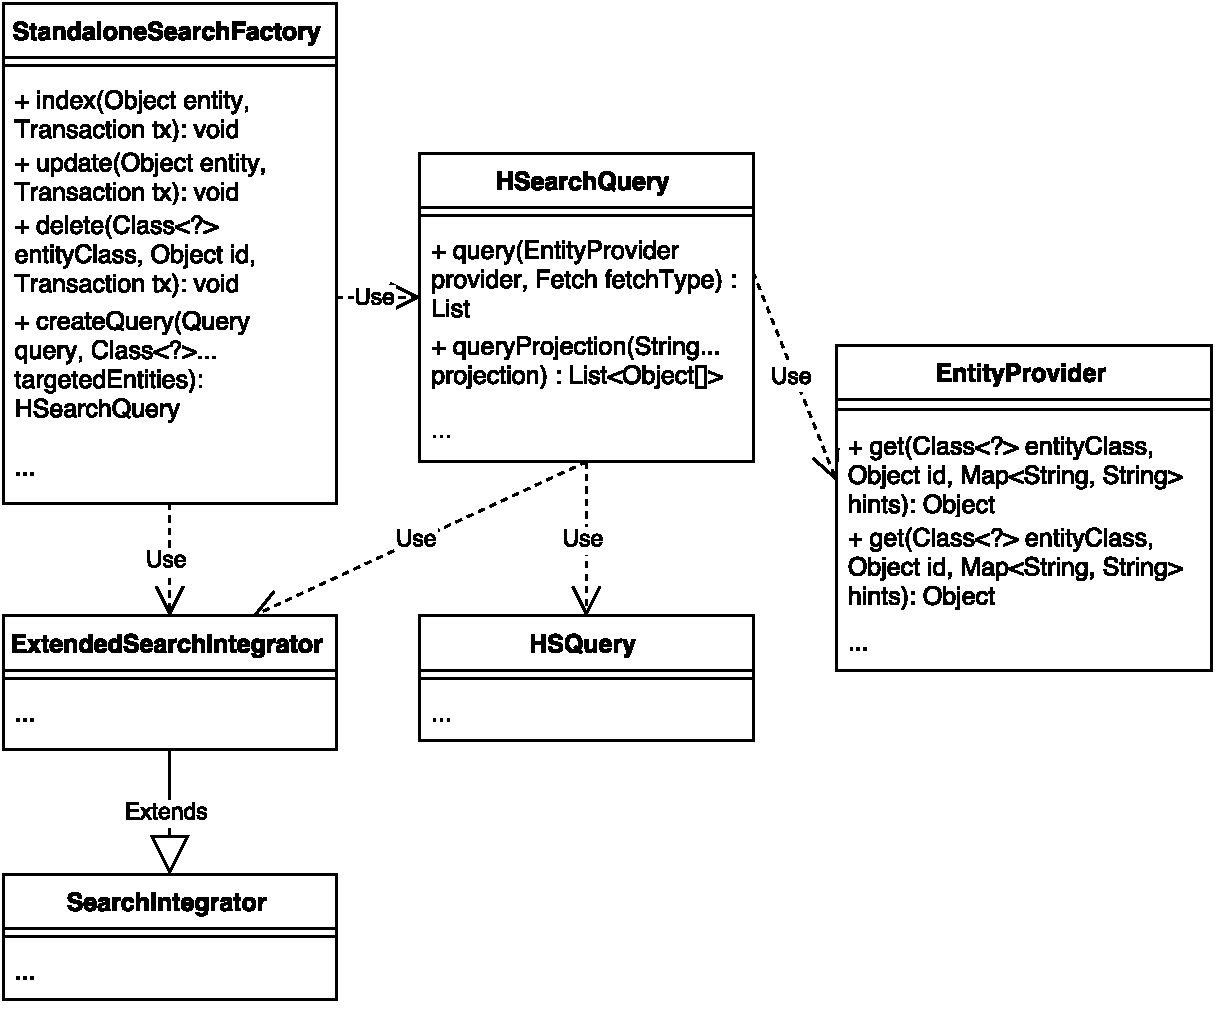
\includegraphics[scale=0.6]{images/standalone_min_architecture.pdf}
	\caption{Rough architecture of the standalone (important parts)}
	\label{standalone_min_architecture}
\end{figure}

\subsubsection{Starting the standalone}

The startup process of the standalone doesn't differ much from manually using the engine in terms of configuration as we still have to use the SearchConfiguration interface. The only different thing is how we build the StandaloneSearchFactory. This is done with a \textbf{StandaloneSearchFactoryFactory}, so the code using it doesn't have to handle the creation of an the actual implementation object.
\\
\lstset{language=java}
\lstset{moredelim=[is][\bfseries]{[*}{*]}}
\begin{lstlisting}[frame=htrbl, caption={Starting up the standalone}, label={lst:using_standalone.java}]
List<Class<?>> indexClasses = Arrays.asList(Book.class, Author.class);

SearchConfiguration searchConfiguration = 
		new StandaloneSearchConfiguration();
indexClasses.forEach( searchConfiguration::addClass );

StandaloneSearchFactory searchFactory = 
		StandaloneSearchFactoryFactory.
				createSearchFactory(
					searchConfiguration,
					indexClasses
				);
				
//use the searchfactory ...

//close it
searchFactory.close();
\end{lstlisting}

\subsubsection{Indexing, updating and deleting objects from the index}

With our standalone version, basic index control becomes more streamlined as we don't have to work with  SearchIntegrator's Worker pattern anymore.
\\
\lstset{language=java}
\begin{lstlisting}[frame=htrbl, caption={Indexing an object with the standalone}, label={lst:indexing_object_native.java}]
Book book = ...;
Transaction tx = new Transaction();
searchFactory.index(book, tx);
tx.commit();
\end{lstlisting}

\lstset{language=java}
\begin{lstlisting}[frame=htrbl, caption={Updating an object with the standalone}, label={lst:updating_object_native.java}]
Book book = ...;
Transaction tx = new Transaction();
searchFactory.update(book, tx);
tx.commit();
\end{lstlisting}

\lstset{language=java}
\begin{lstlisting}[frame=htrbl, caption={Deleting an object by id with the standalone}, label={lst:deleting_object_native.java}]
Transaction tx = new Transaction();
String isbn = ...;
searchFactory.delete(Book.class, isbn, tx);
tx.commit();
\end{lstlisting}

\subsubsection{Querying the index} \label{querying_standalone}
The biggest change in the standalone version is probably how the index is queried. We don't have to work with EntityInfos anymore as we introduce the \textbf{EntityProvider} interface. This interface hosts one method that is to be used for batch fetching (Fetch.BATCH) and one for single fetching (FETCH.FIND\_BY\_ID).
\\\\
A good default implementation delegating the database access to a JPA EntityManager is our \textbf{BasicEntityProvider} (\ref{lst:BasicEntityProvider.java}). Besides taking a EntityManager in its constructor, the class also needs a Map<Class<?>, String> containing the id properties of the entities. While we leave the construction of this map out in the following example for the sake of simplicity, the code for this can be found in the listings (\ref{lst:idProperties.java}). After its creation this map can then be stored in a central place and be reused.
\\
\lstset{language=java}
\begin{lstlisting}[frame=htrbl, caption={Querying the index with the standalone}, label={lst:querying_natively.java}]
StandaloneSearchFactory searchFactory = ...;

EntityManager em = ...;
Map<Class<?>, String> idProperties = ...;

EntityProvider entityProvider = new BasicEntityProvider(em, idProperties);

List<Book> = searchFactory.createQuery(searchFactory.buildQueryBuilder()
				.forEntity(Book.class)
				.get()
				.keyword()
				.onField("title")
				.matching("searchString")
				.createQuery(), Book.class
			).query(
				entityProvider,
				Fetch.BATCH
			);
\end{lstlisting}

\pagebreak

\subsection{Standalone integration with JPA interfaces}
After simplifying the access to Hibernate Search's engine we will work out an integration with JPA interfaces next. Since we started with the premise of not wanting to "reinvent the wheel" by writing everything from scratch - which was one of the reasons why we chose to use Hibernate Search's engine in the first place - we will try to build an integration as similar to the JPA interfaces of Hibernate Search ORM as possible.
\\\\
Before we can go into detail about how we build our integration, we have to discuss the general architecture first. We will go over how the Hibernate Search ORM integration with JPA interfaces behaves from a user point and then take a look at what has to be changed in order to be compatible with any JPA implementor.

\subsubsection{Architecture of Hibernate Search ORM}

Hibernate Search ORM integrates with the JPA API by extending the interfaces  javax.persistence.EntityManager and javax.persistence.Query and adding new functionality to the fulltext search versions of these interfaces: \textbf{FullTextEntityManager} and \textbf{FullTextQuery}. The following figure shows a rough overview of this. Note that this only contains only the methods relevant for the following inspections.
\\
\begin{figure}[ht]
	\centering
	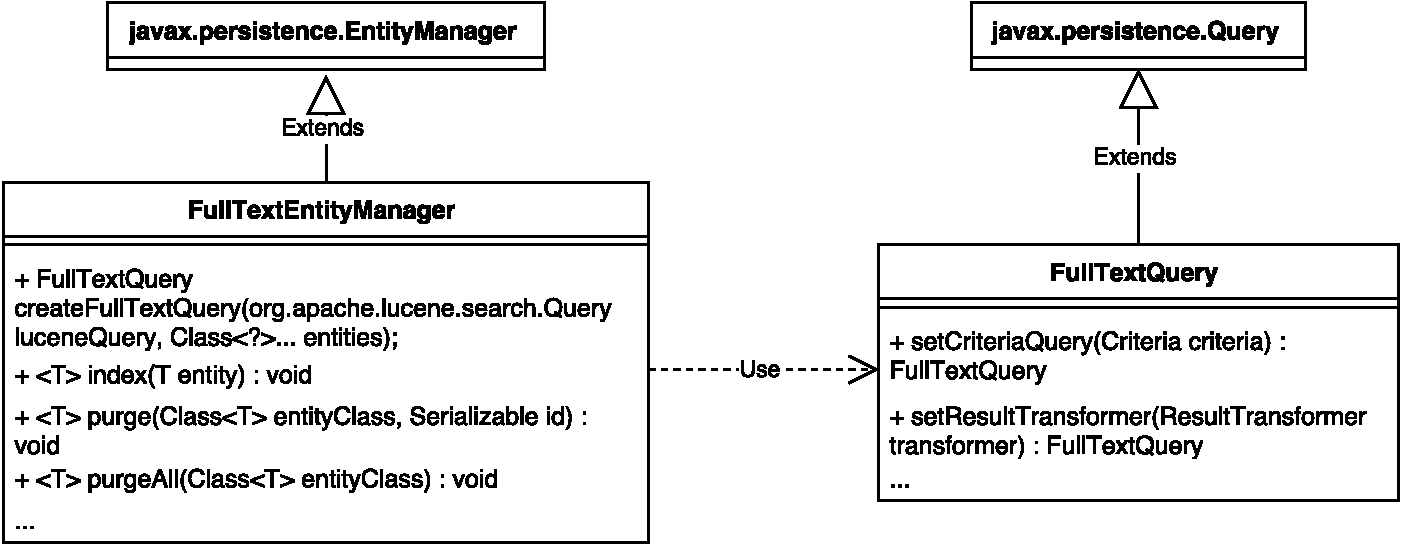
\includegraphics[scale=0.6]{images/hibernate_search_jpa_integration_original.pdf}
	\caption{The main JPA interfaces of Hibernate Search ORM}
	\label{hibernate_search_jpa_integration_original}
\end{figure}

\paragraph{Starting}
As Hibernate Search ORM is tightly coupled with Hibernate ORM it is automatically started if found on the classpath and the persistence.xml contains the following:
\\
\lstset{language=java}
\begin{lstlisting}[frame=htrbl, caption={Additions to persistence.xml with Hibernate Search ORM}, label={lst:hibernate_search_persistence.xml}]
...
<property name="hibernate.search.default.directory_provider"
value="filesystem"/>
<property name="hibernate.search.default.indexBase"
value="/path/to/indexes"/>
...
\end{lstlisting}
\noindent
This means that there exists no real code entry point as Hibernate Search is fully integrated into the Hibernate ORM/OGM lifecycle. FullTextEntityManagers can therefore be obtained with:
\\
\lstset{language=java}
\begin{lstlisting}[frame=htrbl, caption={Obtaining a FullTextEntityManager with Hibernate Search ORM}, label={lst:indexing_object_hsearch_orm_jpa.java}]
EntityManager em = ...;
FullTextEntityManager fem = Search.getFullTextEntityManager(em);
\end{lstlisting}
All of FullTextEntityManager's operations are controlled by the same transactions the original Hibernate EntityManager is using. This is the reason we will not have any search Transaction related code in the following paragraphs.

\paragraph{Indexing, updating and deleting objects from the index}
The index operations are all straightforward and are similar to what we designed our Standalone integration in \ref{standalone_hibernate_search} to work like apart from minor naming differences. 
\\\\
Hibernate Search ORM doesn't differentiate between indexing and updating.
\\
\lstset{language=java}
\begin{lstlisting}[frame=htrbl, caption={Indexing/Updating an object with Hibernate Search ORM}, label={lst:indexing_object_hsearch_orm_jpa.java}]
FullTextEntityManager fem = ...;
Book book = ...;
fem.index(book);
\end{lstlisting}
\noindent
Deleting objects from the index is called purging. This is probably due to not wanting to confuse it with JPA's delete(...).
\\
\lstset{language=java}
\begin{lstlisting}[frame=htrbl, caption={Deleting an object by id with Hibernate Search ORM}, label={lst:deleting_object_hsearch_orm_jpa.java}]
FullTextEntityManager fem = ...;
String isbn = ...;
fem.purge(Book.class, isbn);
\end{lstlisting}

\paragraph{Querying the index} \label{hsearch_orm_querying}
Hibernate Search ORM integrates even better with JPA for queries than our Standalone version as the FullTextQuery interfaces extends the JPA Query interface and uses getResultList() to return its results.
\\
\lstset{language=java}
\begin{lstlisting}[frame=htrbl, caption={Querying with Hibernate Search ORM}, label={lst:querying_hsearch_orm.java_1}]
EntityManager em = ...;
FullTextEntityManager fem = Search.getFullTextEntityManager(em);

FullTextQuery fullTextQuery = fem.createFullTextQuery(
	searchFactory.buildQueryBuilder()
		.forEntity(Book.class)
		.get()
		.keyword()
		.onField("title")
		.matching("searchString")
		.createQuery(), 
	Book.class);
	
List<Book> books = (List<Book>) fullTextQuery.getResultList();
\end{lstlisting}

\paragraph{Index rebuilds}
A noteworthy feature of Hibernate Search is its MassIndexer. It can be used whenever the way the entities are indexed is changed (e.g. in the @Field annotations). It uses multiple threads working in parallel to scroll results from the database and then indexes these efficiently. This is by far faster than the naive approach working in only one thread. It also incorporates a lot of internal improvements a normal developer wouldn't have access to as the specifics are hidden in the implementation packages of Hibernate Search which are not intended to be used outside of its own code.
\\\\
A full index rebuild for our Book entity would look like this:
\\
\lstset{language=java}
\begin{lstlisting}[frame=htrbl, caption={MassIndexer usage with Hibernate Search ORM}, label={lst:massindexing_hsearch_orm.java}]
EntityManager em = ...;
FullTextEntityManager fem = Search.getFullTextEntityManager(em);

fem.createIndexer( Book.class )
	.batchSizeToLoadObjects( 25 )
	.threadsToLoadObjects( 12 )
	.idFetchSize( 150 )
	.transactionTimeout( 1800 )
	.startAndWait();
\end{lstlisting}
\noindent
"This will rebuild the index of all [Book] instances (and subtypes), and will create 12 parallel threads to load the User instances using batches of 25 objects per query; these same 12 threads will also need to process indexed embedded relations and custom FieldBridges or ClassBridges, to finally output a Lucene document."\footnote{Hibernate Search documentation (MassIndexer, v5.4), see~\cite{hibernate_search_doc_massindexer}}

\pagebreak

\subsubsection{Architecture of the generic version}

As good as Hibernate Search ORM's API integration with JPA's EntityManager and Query interface is, its additional interfaces still contain some Hibernate ORM related features and logic that a generic version can not support and therefore have to be changed, emulated or removed all together.
\\
\begin{figure}[ht]
	\centering
	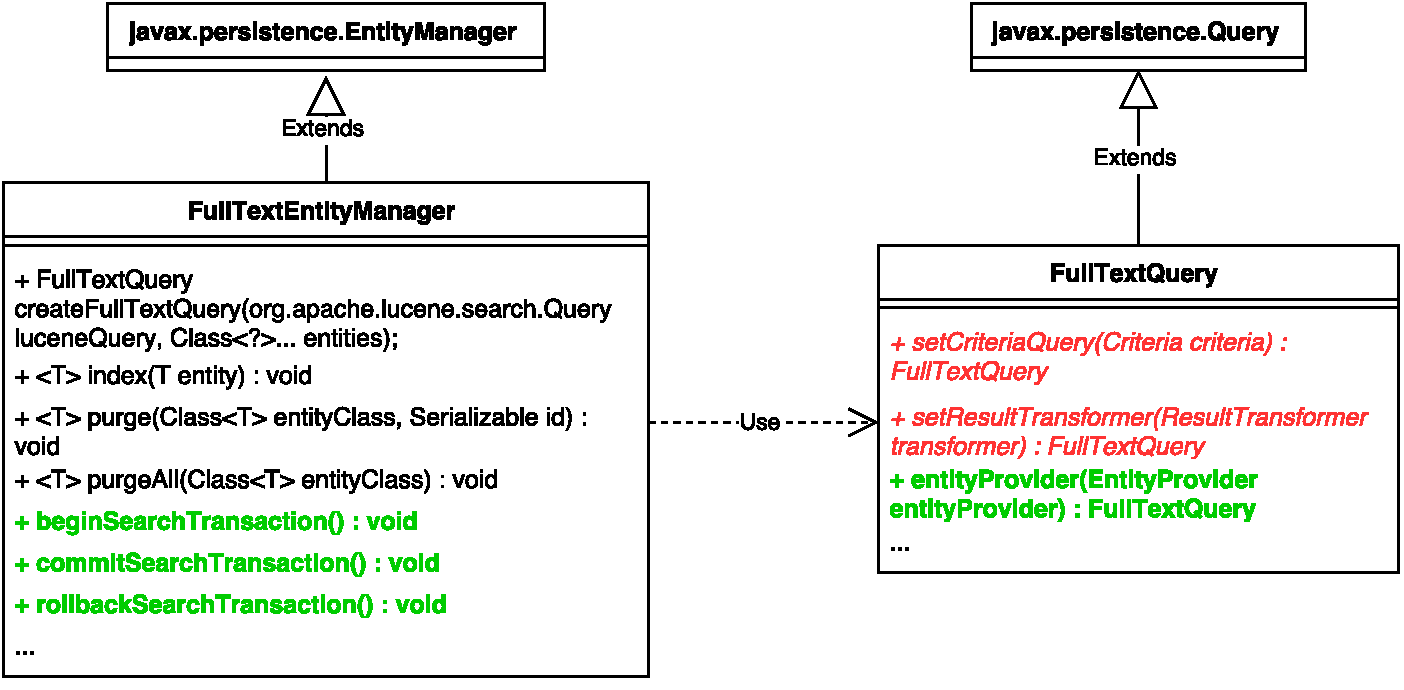
\includegraphics[scale=0.6]{images/hibernate_search_jpa_integration_with_differences.pdf}
	\caption{Required fixes for a generic version}
	\label{hibernate_search_jpa_integration_with_differences}
\end{figure}
\\
In the figure above, we marked all the methods needing fixing in the FullTextEntityManager and FullTextQuery interfaces. Besides these, some other aspects need changing as well. We will discuss all of the needed changes \& additions in the following paragraphs.

\paragraph{Starting}

In our generic version we can't tightly integrate with the EntityManagerFactory of the JPA provider. This is the reason we introduce a separate interface called \textbf{JPASearchFactoryController}.

\begin{figure}[ht]
	\centering
	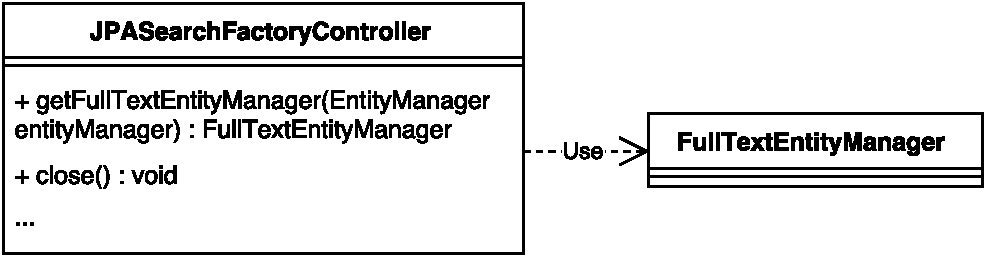
\includegraphics[scale=0.6]{images/JPASearchFactoryController.pdf}
	\caption{JPASearchFactoryController}
	\label{jpa_searchfactory_controller}
\end{figure}
\noindent
Having this separate interface means that its lifecycle has to be controlled on its own. We start it with our bootstrapping class \textbf{Setup} like this:
\\
\lstset{language=java}
\begin{lstlisting}[frame=htrbl, caption={MassIndexer usage with Hibernate Search ORM}, label={lst:massindexing_hsearch_orm.java}]
EntityManagerFactory emf = ...;
Properties properties = new Properties();

properties.setProperty(
	"hibernate.search.searchfactory.type", 
	"manual-updates"
);

JPASearchFactoryController searchFactoryController =
	Setup.createSearchFactoryController( emf, properties );

//use it...

searchFactoryController.close();
\end{lstlisting}
\noindent
For this example we are using "manual-updates", as we haven't discussed how the index is kept up-to-date. After we worked that out, "manual-updates" will just be a fallback setting for developers not wanting to have the index automatically updated.  Also note that there are many more properties that can be set and vanilla Hibernate Search settings are passed this way as well. A complete list of the available generic jpa configuration properties can be found in table \ref{table:config_properties_jpasearchfactorycontroller} in the appendix.
\\\\
Unlike the static way a FullTextEntityManager is obtained in Hibernate Search ORM via the Search class, in our generic version, we obtain it with the \textbf{getFullTextEntityManager(EntityManager entityManager)} method. This means that an instance of the JPASearchFactoryController has to be available at all times access to the index is required.
\\\\
Using a non-static approach here has one benefit, though: We can pass null to this method and get a search only FullTextEntityManager that can be used to work on the index when no database access is needed. This is particularly useful if we want to index POJOs which are not associated with JPA (see table \ref{table:config_properties_jpasearchfactorycontroller} for the property to work with these additional entities).

\paragraph{Indexing, updating and deleting objects from the index}

In Hibernate Search ORM, all manual index manipulation is synchronized with the EntityManager transaction lifecycle. In our generic approach we cannot do this as JPA doesn't have an extension point for this kind of usage. This is the reason we introduce the \textbf{[begin/commit/rollback]SearchTransaction()} methods in FullTextEntityManager. These have to be used to control the transaction lifecycle of all the index manipulation methods.
\\
\lstset{language=java}
\begin{lstlisting}[frame=htrbl, caption={Index control with Hibernate Search GenericJPA}, label={lst:index_control_hibernatesearchgenericjpa}]
EntityManager em = ...;
JPASearchFactoryController searchFactoryController = ...;

FullTextEntityManager fem = 
	searchFactoryController.getFullTextEntityManager(em);

fem.beginSearchTransaction();
try {
	//index or purge here
	fem.commitSearchTransaction();
} catch(Exception e) {
	fem.rollbackSearchTransaction();
	throw e;
}
\end{lstlisting}
\textcolor{red}{macht eh keinen sinn, da wir eh async backends haben, da sollte dann der user lieber die transactions selber machen}
\\\\
One additional problem with supporting indexing generic JPA entities is that some JPA providers don't return objects of the same Java type the user sees. For example, EclipseLink returns an object of an anonymous subclass of the original in which it hides away some utility logic needed for lazy loading, etc.. But the engine needs to know which class to get the index description metamodel from.
\\\\
This is the reason we implemented logic to feed the right entity class into the engine via user input. Entity classes have to be marked with \textbf{@InIndex} on the type level so we can start from any object's class and then go up in the class hierarchy until we find one that is annotated with this annotation.
\\
\lstset{language=java}
\begin{lstlisting}[frame=htrbl, caption={Algorithm to determine the actual indexed type}, label={lst:algo_subclasssupport}]
// get the first class in the hierarchy that is actually in the index
Class<T> clazz = (Class<T>) entity.getClass();
while ( (clazz = (Class<T>) clazz.getSuperclass()) != null ) {
	if ( clazz.isAnnotationPresent( InIndex.class ) ) {
		break;
	}
}
if ( clazz != null ) {
	return clazz;
}
//no @InIndex found, try this class
return entity.getClass();
\end{lstlisting}
\noindent
Note that this has to be done for every entity that is part of the index, even the ones that are just embedded. With this in mind our entities Book and Author now look like this:
\\
\lstset{language=java}
\begin{lstlisting}[frame=htrbl, caption={Book.java with @InIndex}, label={lst:book.java_2}]
@Entity
@InIndex
@Table(name = "Book")
public class Book {
	
	//rest is unchanged

}
\end{lstlisting}

\lstset{language=java}
\begin{lstlisting}[frame=htrbl, caption={Author.java with @InIndex}, label={lst:author.java_2}]
@Entity
@InIndex
@Table(name = "Author")
public class Author {
	
	//rest is unchanged
	
}
\end{lstlisting}

\paragraph{Querying the index}
While we didn't mention this in \ref{hsearch_orm_querying}, Hibernate Search ORM supports modifying the resulting objects of a query with these two methods:

\begin{itemize}
	\item \textbf{setCriteriaQuery(Criteria criteria)}:
		This method lets the user define a custom Hibernate Criteria query (no JPA criteria query) that has to be used to retrieve the results from the database. This can be used to make sure all necessary data is loaded after it is returned by getResultList(). These custom queries are  particularly in cases where no session is available when the data is actually used: If the data is requested, an error would occur.
	\item \textbf{setResultTransformer(ResultTransformer resultTransformer)}:
		A ResultTransformer can be used to transform the results (useful for projections) into POJOs (Plain Old Java Object).
\end{itemize}
\noindent
There is a problem with these two methods, though. They are using the Hibernate ORM API to accomplish their behaviour, and therefore we cannot support them.
\\\\
By adding a new method \textbf{entityProvider(EntityProvider entityProvider)} with the same EntityProvider interface as in \ref{querying_standalone} to the method, we can at least support custom queries. 
\\\\
As the main use case scenario for the ResultTransformer is probably just the transformation from a projection of the queried documents to a POJO, we just completely remove this feature. In the future, we can add such a feature back to the generic version, if needed. But as this method cannot be kept as-is anyways, Hibernate Search ORM developers switching to the generic version that use this feature have to change some of their code either way.

\paragraph{Index rebuilds}

\subsubsection{Implementation Details}

-> SubClassSupportInstanceInitializer, MassIndexer, Transaction Management





-> 


\pagebreak

% !TeX spellcheck = en_GB
\subsection{The automatic index updating feature}

As already stated in \ref{automatic_indexing_problematic_intro}, the automatic index updating feature is a required for a reasonable Hibernate Search GenericJPA. As this is arguably the most complicated feature for GenericJPA, we will go into detail about how we are achieving it compared to the short introductions of the other features.

\subsubsection{Description of different implementations} \label{description_of_different_implementations}

There are several approaches to building an automatic index updating feature. While they are all different in the specifics, they can generally be separated into two categories: \textbf{synchronous} and \textbf{asynchronous}. Synchronous in this context means that the index is updated as soon as the newly changed data is persisted in the database without any real delay while in an asynchronous updating mechanism an arbitrary amount of time passes before the index is updated. While synchronous approaches are needed in some rare cases, fulltext search generally doesn't require a 100\% up-to-date at every point in time index as a search index generally is not the source of truth in an application (only the database contains the "truth").
\\\\
We will now work out a solution for both sync and async, while the async version will serve as a backup whenever the synchronized mechanism is not applicable.

\pagebreak

\paragraph{Synchronous approach}

For the synchronous approach we have two candidates: A system based on JPA callback events and another one that uses the native APIs of JPA providers. We start with the JPA callbacks and then go onto the native APIs.

\subparagraph{JPA events}

As we are trying to work with as little vendor specific APIs, JPA's callback events looks like a suitable candidate for listening to changes in entities.
\\\\
To listen for the JPA events we have two options: annotate the entities with callback methods or create a separate listener class. We will only take a look at the listener class since we don't want to have unnecessary methods in a possible user's entities. This class doesn't have to implement an interface, but has to have methods annotated with special annotations. The relevant ones are @PostPersist, @PostUpdate, @PostDelete (there are "pre-versions" available as well, but we focus on the post methods as they are more useful). What each specific annotation stands for is quite self-explanatory.
\\\\
Such a class generally looks like this:
\\
\lstset{language=java}
\lstset{moredelim=[is][\bfseries]{[*}{*]}}
\begin{lstlisting}[frame=htrbl, caption={Example JPA entity listener}, label={lst:jpa_entity_listener.java}]
public class EntityListener {

	@PostPersist
	public void persist(Object entity) {
		//handle the event
	}
	
	@PostUpdate
	public void update(Object entity) {
		//handle the event
	}
	
	@PostDelete
	public void delete(Object entity) {
		//handle the event
	}

}
\end{lstlisting}
\noindent
It is then applied with an annotation on the entity:
\\
\lstset{language=java}
\lstset{moredelim=[is][\bfseries]{[*}{*]}}
\begin{lstlisting}[frame=htrbl, caption={Using a JPA entity listener}, label={lst:using_jpa_entitylisteners.java}]
[*@EntityListeners( { EntityListener.class } )*]
public class Book {

	//...

}
\end{lstlisting}
\noindent
As the JPA provider creates the EnityListeners automatically, we have no access to them without injecting a reference to them in a static way. While this might cause some Classloader problems, it should be fine in most cases.
\\
\lstset{language=java}
\lstset{moredelim=[is][\bfseries]{[*}{*]}}
\begin{lstlisting}[frame=htrbl, caption={Injecting the EntityListener}, label={lst:jpa_entity_listener.java}]
public class EntityListener {

	public EntityListener() {
		// inject it somewhere
		// so we can access it in a static way
		EntityListenerRegistry.inject(this);
	}

	//...

}
\end{lstlisting}

\noindent
Even though these listeners seem to be the perfect fit as they would enable us to fully integrate only with JPA interfaces, they have two big issues as we find out after investigating further.
\\\\
Firstly, not all JPA providers seem to handle these events similar: For example Hibernate ORM doesn't propagate events from collection tables to the owning entity, while EclipseLink does (EclipseLink's behaviour would be needed from all providers).
\\\\
Secondly, we can see that the events are triggered on flush instead of commit. This is an issue if the changed data is not actually commited.
\\

\lstset{language=java}
\lstset{moredelim=[is][\bfseries]{[*}{*]}}
\begin{lstlisting}[frame=htrbl, caption={Event triggering on flush}, label={lst:flush_event.java}]
EntityManager em = ...;

em.getTransaction().begin();

Book book = em.find( Book.class "someIsbn" );
book.setTitle( "someNewTitle" );

// flushes, so we retrieve the Book with the changes from above
// => event is triggered
List<Book> allBooks = 
	em.createQuery( "SELECT b FROM Book b" ).getResultList();

// we have no way to get this event to revert the wrong index change
em.getTransaction().rollback();
\end{lstlisting}

\noindent
While it \textbf{might} be possible to somehow fix the flush issue, the bad support from JPA providers like Hibernate ORM renders this approach unusable until the JPA providers work the same way to some reasonable extent.

\subparagraph{Native integration with JPA providers}

Almost every JPA provider has its own internal event system that is useful for cache invalidation and other tasks. These combined with hooks into the transaction management allow us to build a proper index updating system that works with transactions in mind (big improvement compared to the flush() issues of plain JPA)
\\\\
They generally have callbacks similar to these of the JPA events (no knowledge about database specifics is needed, Java types are used), but also provide additional information about the database session that caused the changes.
\\\\
By definition, these kind of integrations are not portable between JPA providers and require us to write different systems for all the JPA providers. But as the landscape for popular JPA providers probably only consists of Hibernate ORM, EclipseLink and OpenJPA, we can implement listeners for these and the others will have to rely on the async backup approach (as of the time of writing this, we have only implemented integrations for Hibernate ORM and EclipseLink).
\\\\
As this seems to be the only reasonable solution for a synchronous update system, we are using it for Hibernate Search GenericJPA.
\\\\
\textit{Note: we don't describe how these event systems are built in particular as they differ a lot in their APIs, but generally these are straightforward to use and describing the implementations would be unspectacular.}

\pagebreak

\paragraph{Asynchronous approach}
In contrary to the synchronous approach where we described two different versions, for the asynchronous version we only have one feasible solution available: A trigger based system.
\\\\
Triggers are "procedural code that is automatically executed in response to certain events on a particular table or view in a database" \footnote{Wikipedia on RDBMS triggers, see~\cite{triggers_wiki}}. While they are mostly "used for maintaining the integrity of the information on the database" \footnote{Wikipedia on RDBMS triggers, see~\cite{triggers_wiki}}, they are also useful for listening to events.
\\\\
Almost every RDBMS at least supports triggers on the three crucial events for event-listening: INSERT (CREATE), UPDATE, DELETE.
\\\\
In order to have triggers being useful for updating our Hibernate Search index, we have to get info about the events from the database back into our Java application. Since we cannot necessarily call Java code from our database (with the exception of some enterprise and in-memory databases), we have to write data about changes into auxiliary tables and then poll these regularly.
\\\\
One benefit of this approach is that by using polling from the tables and the - by definition transactional - triggers, we don't have to hook into transactions or deal with data that has not been committed, yet, in general. If we do things right, we can even improve indexing performance by this: We can query for the latest event for each entity only, so we don't use up an unnecessary amount of CPU-time we don't need, but still keep the index up-to-date.

\subparagraph{Trigger architecture}

Triggers are generally created on tables. Since we want to use them for event-listening, we have to cover every table of the domain model that contains data indexed/stored in the index. This also includes all of the mapping tables between entities and all other secondary tables.
\\\\
The following figure shows the trigger architecture needed for our Author and Book example.

\pagebreak

\begin{figure}[ht]
	\centering
	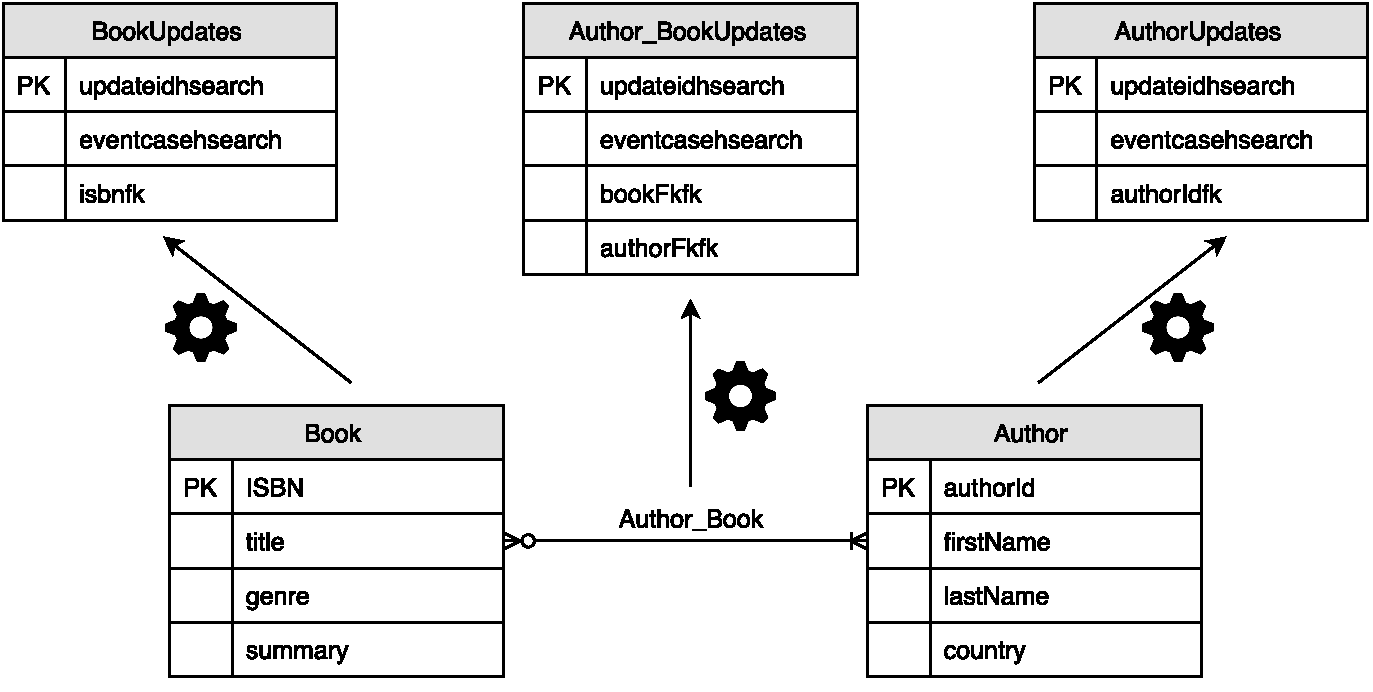
\includegraphics[scale=0.6]{images/Triggers_Schema.pdf}
	\caption{Triggers for the example project}
	\label{triggers_schema}
\end{figure}
\noindent
All three tables Author, Book and Author\_Book have three triggers registered on them (one for each event type). These triggers then fill up the update tables AuthorUpdates, BookUpdates and Author\_BookUpdates (these names are just for demonstrative purposes) with info about occurring events. We can see that these update tables host at least three things:

\begin{enumerate}
	\item \textbf{updateid primary key:} Update events have to be sortable by the order they occured. All Update tables share the same sequence of primary keys so that no key appears twice in all of these tables.
	\item \textbf{eventcase column:} This column contains a identifier for the cases INSERT, DELETE or UPDATE.
	\item \textbf{pseudo foreign key(s):} The relevant primary keys of the entities involved in the tables have to be stored in the Update tables as well. Note that they are not marked as real foreign keys as a DELETE event wouldn't work then (we can't have a reference to a non existent entity).
\end{enumerate}

\subparagraph{Creating the tables} \label{creating_the_tables}

Since the creation of these tables requires a lot of work to be done, we have to automate it as good as possible. We do this by requiring additional annotations on the entities to map the required information for the update tables and then generating them out of it.
\\\\
These annotations contain at least the original table's name and the types \& names of the entity key columns. The name of the update table and the columns in it is then generally derived automatically from that.
\\\\
\textit{Note: The update tables are NO JPA entities, so we have to work with native SQL in the backend}
\\
\lstset{language=java}
\lstset{moredelim=[is][\bfseries]{[*}{*]}}
\begin{lstlisting}[frame=htrbl, caption={Book.java with Hibernate Search annotations}, label={lst:book.java_3}]
@Entity
@InIndex
@Table(name = "Book")
@Indexed
[*@UpdateInfo(
	tableName = "Book", 
	idInfos = 
	@IdInfo(columns = 
		@IdColumn(
			column = "isbn", 
			columnType = ColumnType.STRING
		)
	)
)*]
public class Book {

	// ... unchanged. 
	
	//mapping table events handled on Author side
	
	//getters & setters ...
}
\end{lstlisting}

\lstset{language=java}
\lstset{moredelim=[is][\bfseries]{[*}{*]}}
\begin{lstlisting}[frame=htrbl, caption={Author.java with Hibernate Search annotations}, label={lst:author.java_3}]
@Entity
@InIndex
@Table(name = "Author")
[*@UpdateInfo(
	tableName = "Author", 
	idInfos = 
	@IdInfo(columns = 
		@IdColumn(
			column = "authorId", 
			columnType = ColumnType.LONG
		)
	)
)*]
public class Author {
	
	// ... unchanged.
	
	[*@UpdateInfo(tableName = "Author_Book", 
		idInfos = {
		@IdInfo(entity = Author.class, 
			columns = 
			@IdColumn(
				column = "authorFk",
				columnType = ColumnType.LONG
			)
		),
		@IdInfo(entity = Book.class,
			columns = 
			@IdColumn(
				column = "bookFk",
				columnType = ColumnType.STRING
			)
		)
	})*]
	private Set<Book> books;
	
	//getters & setters ...
}
\end{lstlisting}
\noindent
However, if the developer needs different names in the update tables, it is possible to manually set these properties. They can be found on the same level as the corresponding info for the original table is set.
\\\\
Options for multivalued keys and custom column types are also available as by default only singular valued keys of the column types corresponding to Java's Integer, Long and String are supported. While we don't go into detail how these expert features are used, information about how to use them can be found in the Javadoc of the annotations.
\\\\
Since database triggers and tables are not created the same on every RDBMS, we have to build an abstraction to get the necessary SQL code. This is done with the \textbf{TriggerSQLStringSource} interface. Its implementations return the specific SQL strings working on the corresponding RDBMS. As of this writing we have implementations for MySQL, PostgreSQL and HSQDLB. See table \ref{table:config_properties_jpasearchfactorycontroller} for information about using these.
\\\\
Whether and how the triggers and tables are generated at all can also be set, but with a configuration property on the SearchFactoryController as described in table  \ref{table:config_properties_jpasearchfactorycontroller}. If disabled, the user still has to provide the information about the update tables that should be used for updating with the annotations as described above.

\subparagraph{Retrieving the events}
Now that we know how the events are stored in the update tables, we will now describe an efficient way to query the database for these entries.
\\\\
We only need the latest event for each entity (or combination of entities for mapping tables). The following SQL query is doing this for the table author\_bookupdates with standard SQL that should be working on every RDBMS.
\\
\lstset{language=sql}
\lstset{moredelim=[is][\bfseries]{[*}{*]}}
\begin{lstlisting}[frame=htrbl, caption={Querying for updates (Author\_Book)},
label={lst:querying_updates.sql}]
SELECT t1.updateidhsearch, t1.authorFkfk, t1.bookFkfk
FROM author_bookupdates t1
INNER JOIN
(
	/* select the most recent update */
	SELECT max(t2.updateidhsearch) updateid, 
		t2.authorFkfk, t2.bookFkfk
	FROM author_bookupdates t2
	GROUP BY t2.authorFkfk, t2.bookFkfk
) t3 on t1.updateidhsearch = t3.updateid
/* handle events that occured earlier first */
ORDER BY t1.updateidhsearch ASC;
\end{lstlisting}
\noindent
We run queries of this type for every update table with fixed delays (configurable, see table \ref{table:config_properties_jpasearchfactorycontroller}). Then, we scroll from the results
of these queries simultaneously while ordering by the updateids between the queries to make sure the events are definitely handled in the right order (see listing \ref{lst:MultiQueryAccess.java} in the appendix).
\\\\
This information is all we need to keep our index up-to-date. For the INSERT and UPDATE case we can just query the database for a new version and pass that to the engine. For the DELETE case we have to work directly on the index and have to enforce  \textbf{@IndexedEmbedded\#includeEmbeddedObjectId = true}. This is required so that we can determine the root entity in the index as its entry has to be updated additionally if the original entity is changed (A entity contained in one index can have its own index as well).
\\\\
After the index is updated accordingly, we run a delete query that deletes all update events
having an updateid lower than the last processed one for each table.
\\
\lstset{language=sql}
\lstset{moredelim=[is][\bfseries]{[*}{*]}}
\begin{lstlisting}[frame=htrbl, caption={Deleting handled updates (Author\_Book)},
label={lst:deleting_updates.sql}]
DELETE FROM author_bookupdates WHERE updateidhsearch < #last_handled_id#
\end{lstlisting}
\noindent
With these two types of queries for each update table we are able to keep the index up-to-date efficiently and also make sure that no event is handled twice.

\pagebreak

\subsubsection{Comparison of approaches}

We already discussed the differences of synchronous and asynchronous approaches in general earlier this chapter. The two chosen implementations differ in terms of extra work that has to be done to get them to work (user-friendliness for the developer) and features.

\paragraph{Additional work}
Since the native event system gets the proper information about changes from the vendor side, it doesn't require a lot information about the general structure of the domain model and tables in the database. For the Trigger based event system, that's a different story as it has to poll info about changes from the database. This is the reason the user has to add this information as we have seen in \ref{creating_the_tables}.
\\
\begin{figure}[ht]
	\centering
	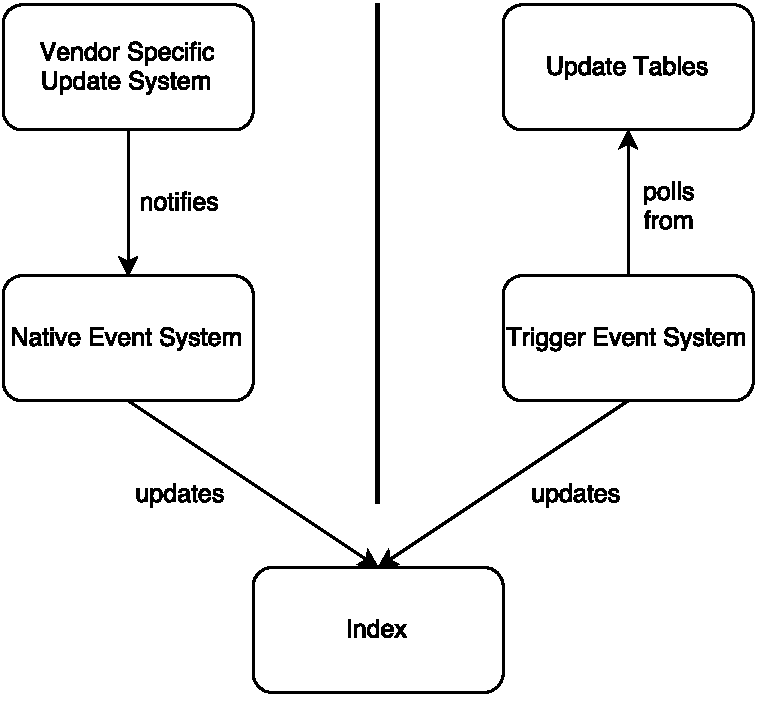
\includegraphics[scale=0.6]{images/UpdateConsumer_Architecture.pdf}
	\caption{Hibernate Search GenericJPA update mechanisms}
	\label{updateconsumer_architecture}
\end{figure}

\paragraph{Features}
The native event system has the exact same updating behaviour as Hibernate Search ORM's update mechanism because it works on the same principles of using the existing event APIs. It just works for more ORM providers.
\\\\
With this similarity come two important drawbacks:
\begin{enumerate}
	\item It (the mechanism) only works with specifically supported JPA APIs
	\item Database changes coming from anything else than JPA APIs are not recognized. This includes native SQL queries from EntityManagers. This also means that the database can only be used by the JPA application and no other scripts, small programs etc. should have write access to the database.
\end{enumerate}
\noindent
These two drawbacks are non-existent with the trigger event system as it doesn't require any specific JPA implementation (1) and works on the database level (2).

\paragraph{Conclusion}
We can see that both event systems can be useful in different cases. This is the reason we use both in Hibernate Search GenericJPA. The following table summarizes the pros and cons once again:

\begin{table}[h] 
	\centering
	\begin{tabular}{|c|c|c|}
		\hline 
		Approach & Pros & Cons \\ 
		\hline 
		\specialcell{Native Event System} & 
		\specialcell{+ No additional work \\ needed by the developer} & 
		\specialcell{- Relies on different\\ implementation- \\ specific APIs \\ (only works with \\ specifically supported ones) \\
					- Changes from outside\\ of the JPA provider \\are not recognized \\ (e.g. native SQL access)} \\ 
		\hline
		\specialcell{Trigger Event System} & 
		\specialcell{+ Works with any JPA \\implementation \\ (even rarely used ones) \\
					+ Changes from outside\\ of the JPA provider \\ are recognized \\ (e.g. native SQL access)} & 
		\specialcell{- Additional work by \\the developer needed \\ (annotations)} \\ 
		\hline
	\end{tabular}
	\footnotesize \caption{Pros and Cons of the two update systems}
	\label{table:pros_and_cons_update_systems}
\end{table}

\pagebreak

% !TeX spellcheck = en_GB
\section{Outlook}\label{outlook}

In this thesis we described how we can integrate Hibernate Search with JPA conform ORM implementations. We started by building a standalone integration of hibernate-search-engine, then integrated it with JPA and finally created an automatic index updating mechanism. All challenges described in \ref{Challenges} have been resolved.
\\\\
The only feature needing some extra work is probably the generic updating mechanism with database triggers. At the moment the developer has to specify additional annotations containing information about the update tables by hand. At least some of the info is known to be able to be retrieved from the JPA provider (via specific interfaces, Hibernate ORM and EclipseLink definitely have this option, others have not been checked). These automatic mechanisms could not be included in this thesis as they would have required a lot more time than was available.
\\\\
During the process of designing and writing the code for Hibernate Search GenericJPA we tried to be as compatible with the orginal Hibernate Search API as possible. While one reason for this is to make the switch easier for developers that want to try it out, the biggest one is that the ultimate goal for this project is to be merged into the original Hibernate Search codebase even though we haven't mentioned this in the beginning.
\\\\
This is also why this project has to be looked as a proof of concept even though the code as it can be found on GitHub \footnote{Hibernate Search GenericJPA GitHub repository, see~\cite{hibernate_genericjpa_github}} can already be used in real applications. In fact as described in \ref{Methods} every relevant part of Hibernate Search GenericJPA has been extensively tested in single feature-tests and integration-tests and can therefore be considered stable. 
\\\\
The first steps of the merging process have already been discussed with the Hibernate Search development team and work on the merging process is to be started in early October 2015. This comes exactly at the right moment as the Hibernate Search team is planning API changes in the near future and \footnote{Hibernate Search roadmap, see~\cite{hibernate_search_roadmap}} some interfaces have to be altered (as seen in \ref{integration_jpa}) in order to support generic JPA.
\\\\
As soon as the generic version is part of Hibernate Search and is fully compatible with its API, Hibernate Search can be looked at as a standard for fulltext search in JPA. Having such a standard would be quite beneficial for the ever changing JPA world as smaller JPA providers could have a better chance at getting a bigger user base. And competition has never been a bad thing.


\onecolumn
% einfacher Zeilenabstand
\singlespacing
% Literaturliste soll im Inhaltsverzeichnis auftauchen
%\addcontentsline{toc}{section}{Literaturverzeichnis}
% Literaturverzeichnis anzeigen
%\renewcommand\refname{Literaturverzeichnis}
%\bibliography{Hauptdatei}

%% Index soll Stichwortverzeichnis heissen
% \newpage
% % Stichwortverzeichnis soll im Inhaltsverzeichnis auftauchen
% \addcontentsline{toc}{section}{Stichwortverzeichnis}
% \renewcommand{\indexname}{Stichwortverzeichnis}
% % Stichwortverzeichnis endgueltig anzeigen
% \printindex

\onehalfspacing
% evtl. Anhang
\newpage
\addcontentsline{toc}{section}{Listings}
\fancyhead[L]{Listings} %Kopfzeile links
\section*{Used software}

For the development of Hibernate Search GenericJPA as described in this thesis we have used the following software and libraries (only the most relevant listed here, for more information check the pom.xml files in the GitHub repository \footnote{Hibernate Search GenericJPA GitHub repository, see~\cite{hibernate_genericjpa_github}}):
\\\\
\noindent
Hibernate Search related libraries:
\begin{itemize}
	\item Hibernate Search 5.5.0.Alpha1 (especially hibernate-search-engine)
	\item Infinispan Directory Provider 8.0.0.Beta3
\end{itemize}

\noindent
Databases:
\begin{itemize}
	\item HSQLDB 2.3.3
	\item MySQL Community Edition 5.5
	\item MariaDB 10.0.17
	\item PostgreSQL 9.4.4
\end{itemize}

\noindent
JPA providers:
\begin{itemize}
	\item EclipseLink 2.5.0
	\item Hibernate ORM 4.3.9
	\item OpenJPA 2.4.0
\end{itemize}

\noindent
Application servers:
\begin{itemize}
	\item Glassfish Embedded 4.1
	\item Wildfly 8.2.0.Final
	\item TomEE 1.7.2
\end{itemize}

\noindent
Building tools:
\begin{itemize}
	\item JUnit 4.11
	\item Arquillian 1.1.8.Final
	\item Maven 3.3.1
\end{itemize}

\pagebreak

\section*{Listings}

Following are some interesting classes referenced in the thesis that were too long to fit into the text.
\\

\noindent
\textbf{Transaction.java}:\\
This class is the simple Transaction representation used to control index changes. It is not intended to be similar to a RDBMS transaction, but is merely a batch context with simple commit and rollback features.
\\
\lstset{language=java}
\begin{lstlisting}[frame=htrbl, caption={the simple Transaction contract}, label={lst:Transaction.java}]
public class Transaction implements TransactionContext {

	private boolean progress = true;
	private List<Synchronization> syncs = new ArrayList<>();
	
	@Override
	public boolean isTransactionInProgress() {
		return this.progress;
	}
	
	@Override
	public Object getTransactionIdentifier() {
		return this;
	}
	
	@Override
	public void registerSynchronization(
		Synchronization synchronization ) {
		this.syncs.add( synchronization );
	}
	
	/**
	 * @throws IllegalStateException if already commited/rolledback
	 */
	public void commit() {
		if ( !this.progress ) {
			throw new IllegalStateException( 
			"can't commit - " + 
			"No Search Transaction is in Progress!" );
		}
		this.progress = false;
		this.syncs.forEach( Synchronization::beforeCompletion );
		
		for ( Synchronization sync : this.syncs ) {
			sync.afterCompletion( Status.STATUS_COMMITTED );
		}
	}
	
	/**
	 * @throws IllegalStateException if already commited/rolledback
 	 */
	public void rollback() {
		if ( !this.progress ) {
			throw new IllegalStateException( 
			"can't rollback - " + 
			"No Search Transaction is in Progress!" );
		}
		this.progress = false;
		this.syncs.forEach( Synchronization::beforeCompletion );
	
		for ( Synchronization sync : this.syncs ) {
			sync.afterCompletion( Status.STATUS_ROLLEDBACK );
		}
	}

}
\end{lstlisting}

\pagebreak

\lstset{language=java}
\begin{lstlisting}[frame=htrbl, caption={StandaloneSearchConfiguration.java}, label={lst:StandaloneSearchConfiguration.java}]
/**
 * Manually defines the configuration. 
 * Classes and properties are the only implemented options at the moment.
 *
 * @author Martin Braun (adaption), Emmanuel Bernard
 */
public class StandaloneSearchConfiguration 
	extends SearchConfigurationBase 
	implements SearchConfiguration {

	private final Logger LOGGER = 
		Logger.getLogger( 
			StandaloneSearchConfiguration.class.getName() 
		);
		
	private final Map<String, Class<?>> classes;
	private final Properties properties;
	private final HashMap<Class<? extends Service>, Object> 
		providedServices;
	private final InstanceInitializer initializer;
	private SearchMapping programmaticMapping;
	private boolean transactionsExpected = true;
	private boolean indexMetadataComplete = true;
	private boolean idProvidedImplicit = false;
	private ClassLoaderService classLoaderService;
	private ReflectionManager reflectionManager;

	public StandaloneSearchConfiguration() {
		this( new Properties() );
	}

	public StandaloneSearchConfiguration(Properties properties) {
		this( 
			SubClassSupportInstanceInitializer.INSTANCE, 
			properties
		);
	}

	public StandaloneSearchConfiguration(InstanceInitializer init) {
		this( new Properties() );
	}

	public StandaloneSearchConfiguration(InstanceInitializer init, 
		Properties properties) {
		this.initializer = init;
		this.classes = new HashMap<>();
		this.properties = properties;
		// default values if nothing was explicitly set
		this.properties.computeIfAbsent(
			"hibernate.search.default.directory_provider", 
			(key) -> {
				LOGGER.info( 
				  "defaulting to RAM directory-provider" 
				);
			return "ram";
		});
		this.properties.computeIfAbsent(
			"hibernate.search.lucene_version", 
			(key) -> {
				LOGGER.info( 
					"defaulting to Lucene Version: " 
					+ Version.LUCENE_4_10_4.toString() 
				);
				return Version.LUCENE_4_10_4.toString();
		});
		this.reflectionManager = new JavaReflectionManager();
		this.providedServices = new HashMap<>();
		this.classLoaderService = new DefaultClassLoaderService();
	}

	public StandaloneSearchConfiguration addProperty(String key,
		String value) {
		properties.setProperty( key, value );
		return this;
	}

	public StandaloneSearchConfiguration addClass(Class<?> indexed) {
		classes.put( indexed.getName(), indexed );
		return this;
	}

	@Override
	public Iterator<Class<?>> getClassMappings() {
		return classes.values().iterator();
	}

	@Override
	public Class<?> getClassMapping(String name) {
		return classes.get( name );
	}

	@Override
	public String getProperty(String propertyName) {
		return properties.getProperty( propertyName );
	}

	@Override
	public Properties getProperties() {
		return properties;
	}

	@Override
	public ReflectionManager getReflectionManager() {
		return this.reflectionManager;
	}

	@Override
	public SearchMapping getProgrammaticMapping() {
		return programmaticMapping;
	}

	public StandaloneSearchConfiguration setProgrammaticMapping(
			SearchMapping programmaticMapping
		) {
		this.programmaticMapping = programmaticMapping;
		return this;
	}

	@Override
	public Map<Class<? extends Service>, Object> 
		getProvidedServices() {
		return providedServices;
	}

	public void addProvidedService(
			Class<? extends Service> serviceRole,
			Object service
		) {
		providedServices.put( serviceRole, service );
	}

	@Override
	public boolean isTransactionManagerExpected() {
		return this.transactionsExpected;
	}

	public void setTransactionsExpected(
			boolean transactionsExpected) {
		this.transactionsExpected = transactionsExpected;
	}

	@Override
	public InstanceInitializer getInstanceInitializer() {
		return initializer;
	}

	@Override
	public boolean isIndexMetadataComplete() {
		return indexMetadataComplete;
	}

	public void setIndexMetadataComplete(
		boolean indexMetadataComplete) {
		this.indexMetadataComplete = indexMetadataComplete;
	}

	@Override
	public boolean isIdProvidedImplicit() {
		return idProvidedImplicit;
	}

	public StandaloneSearchConfiguration 
		setIdProvidedImplicit(boolean idProvidedImplicit) {
		this.idProvidedImplicit = idProvidedImplicit;
		return this;
	}

	@Override
	public ClassLoaderService getClassLoaderService() {
		return classLoaderService;
	}

	public void setClassLoaderService(
		ClassLoaderService ) {
		this.classLoaderService = classLoaderService;
	}

}
\end{lstlisting}

\pagebreak

\lstset{language=java}
\begin{lstlisting}[frame=htrbl, caption={BasicEntityProvider.java}, label={lst:BasicEntityProvider.java}]
public class BasicEntityProvider implements EntityProvider {

	private static final String QUERY_FORMAT = 
		"SELECT obj FROM %s obj " +
		"WHERE obj.%s IN :ids";
	private final EntityManager em;
	private final Map<Class<?>, String> idProperties;

	public BasicEntityProvider(EntityManager em,
		Map<Class<?>, String> idProperties) {
		this.em = em;
		this.idProperties = idProperties;
	}

	@Override
	public void close() throws IOException {
		this.em.close();
	}

	@Override
	public Object get(Class<?> entityClass, Object id,
		Map<String, String> hints) {
		return this.em.find( entityClass, id );
	}

	@SuppressWarnings({"rawtypes", "unchecked"})
	@Override
	public List getBatch(Class<?> entityClass, List<Object> ids,
		Map<String, String> hints) {
		List<Object> ret = new ArrayList<>( ids.size() );
		if ( ids.size() > 0 ) {
			String idProperty = 
				this.idProperties.get( entityClass );
			String queryString = 
				String.format(
					QUERY_FORMAT,
					this.em.getMetamodel()
						.entity( entityClass )
						.getName(),
					idProperty
		);
		Query query = this.em.createQuery( queryString );
		query.setParameter( "ids", ids );
			ret.addAll( query.getResultList() );
		}
		return ret;
	}
	
	public void clearEm() {
		this.em.clear();
	}

	public EntityManager getEm() {
		return this.em;
	}

}
\end{lstlisting}

\pagebreak

\lstset{language=java}
\begin{lstlisting}[frame=htrbl, caption={Obtaining idProperties}, label={lst:idProperties.java}]
SearchConfiguration config = ...;

MetadataProvider metadataProvider = 
	MetadataUtil.getDummyMetadataProvider( config );
MetadataRehasher rehasher = new MetadataRehasher();

List<RehashedTypeMetadata> rehashedTypeMetadatas = new ArrayList<>();
for ( Class<?> indexRootType : this.getIndexRootTypes() ) {
	RehashedTypeMetadata rehashed = 
		rehasher.rehash( 
			metadataProvider
				.getTypeMetadataFor( indexRootType ) 
		);
	rehashedTypeMetadatas.add( rehashed );
}

Map<Class<?>, String> idProperties = 
	MetadataUtil.calculateIdProperties( rehashedTypeMetadatas );
\end{lstlisting}

\pagebreak

\lstset{language=java}
\begin{lstlisting}[frame=htrbl, caption={generic JPA FullTextEntityManager}, label={lst:FullTextEntityManager.java_generic}]
/**
 * @author Emmanuel Bernard
 * @author Martin Braun
 */
public interface FullTextEntityManager extends EntityManager {
	
	/**
	 * Create a fulltext query on top of a native Lucene
	 * query returning the matching objects of columnTypes
	 * <code>entities</code> and their respective subclasses.
	 *
	 * @param luceneQuery The native Lucene query to be 
	 *		run against the Lucene index.
	 * @param entities List of classes for columnTypes filtering.
	 *		The query result will only return entities 
	 *		of the specified types and their respective
	 *		subtype. 
	 *		If no class is specified no columnTypes filtering
	 *		will take place.
	 *
	 * @return A <code>FullTextQuery</code> wrapping around the
	 *	native Lucene query.
	 *
	 * @throws IllegalArgumentException if entityType is 
	 * <code>null</code> or not a class or superclass annotated with
	 * <code>@Indexed</code>.
	 */
	FullTextQuery createFullTextQuery(
		org.apache.lucene.search.Query luceneQuery,
		Class<?>... entities);
	
	/**
	 * Force the (re)indexing of a given <b>managed</b> object.
	 * Indexation is batched per search-transaction: if a
	 * transaction is active, the operation will not affect
	 * the index at least until commit.
	 *
	 * @param entity The entity to index
	 *	- must not be <code>null</code>.
	 *
	 * @throws IllegalArgumentException
	 *	if entity is null or not an @Indexed entity
	 * @throws IllegalStateException
	 *	if no search-transaction is in progress
	 */
	<T> void index(T entity);
	
	/**
	 * @return the <code>SearchFactory</code> instance.
	 */
	SearchFactory getSearchFactory();
	
	/**
	 * Remove the entity with the columnTypes 
	 * <code>entityType</code> and the identifier
	 * <code>id</code> from the index. If
	 * <code>id == null</code> all indexed entities
	 * of this columnTypes and its indexed subclasses
	 * are deleted. In this case
	 * this method behaves like {@link #purgeAll(Class)}.
	 *
	 * @param entityType The columnTypes of the 
	 *	entity to delete.
	 * @param id The id of the entity to delete.
	 *
	 * @throws IllegalArgumentException if entityType is 
	 * <code>null</code> or not a class or superclass 
	 * annotated with <code>@Indexed</code>.
	 * @throws IllegalStateException if no 
	 * search-transaction is in progress
	 */
	<T> void purge(Class<T> entityType, Serializable id);
	
	/**
	 * Remove all entities from of particular class
	 * and all its subclasses from the  index.
	 *
	 * @param entityType The class of the entities to remove.
	 *
	 * @throws IllegalArgumentException if entityType is 
	 *	<code>null</code> or not a class or superclass 
	 * annotated with <code>@Indexed</code>.
	 * @throws IllegalStateException if no search-transaction
	 * is in progress
	 */
	<T> void purgeAll(Class<T> entityType);
	
	<T> void purgeByTerm(Class<T> entityType,
		String field,
		Integer val);
	
	<T> void purgeByTerm(Class<T> entityType,
		String field,
		Long val);
	
	<T> void purgeByTerm(Class<T> entityType,
		String field,
		Float val);
	
	<T> void purgeByTerm(Class<T> entityType,
		String field,
		Double val);
	
	<T> void purgeByTerm(Class<T> entityType,
		String field,
		String val);
	
	/**
	 * Flush all index changes forcing Hibernate Search to apply all
	 * changes to the index not waiting for the batch limit.
	 *
	 * @throws IllegalStateException
	 *	if no search-transaction is in progress
	 */
	void flushToIndexes();
	
	/**
	 * <b>different from the original Hibernate Search!</b> <br>
	 * <br>
	 * this has to be called when you want to 
	 * change the index manually!
	 *
	 * @throws IllegalStateException 
	 *	if a search-transaction is already in progress
	 */
	void beginSearchTransaction();
	
	/**
	 * <b>different from the original Hibernate Search!</b> <br>
	 * <br>
	 * this has to be called when you want to 
	 * change the index manually!
	 *
	 * @throws IllegalStateException
	 *	if no search-transaction is in progress
	 */
	void rollbackSearchTransaction();
	
	/**
	 * <b>different from the original Hibernate Search!</b> <br>
	 * <br>
	 * this has to be called when you want to 
	 * change the index manually!
	 *
	 * @throws IllegalStateException
	 *	if no search-transaction is in progress
	 */
	void commitSearchTransaction();
	
	boolean isSearchTransactionInProgress();
	
	/**
	 * @throws IllegalStateException
	 *	if search-transaction is still in progress.
	 *	underlying EntityManager is still closed.
	 */
	void close();
	
	/**
	 * Creates a MassIndexer to rebuild the indexes of some
	 * or all indexed entity types. Instances cannot be reused. Any
	 * {@link org.hibernate.search.indexes.interceptor
	 *	.EntityIndexingInterceptor} registered on the entity 
	 * types are applied: each instance will trigger an
	 * {@link org.hibernate.search.indexes.interceptor
	 *	.EntityIndexingInterceptor#onAdd(Object)}
	 * event from where you can
	 * customize the indexing operation.
	 *
	 * @param types optionally restrict the operation to 
	 *	selected types
	 *
	 * @return a new MassIndexer
	 */
	MassIndexer createIndexer(Class<?>... types);

}
\end{lstlisting}

\pagebreak

\lstset{language=java}
\begin{lstlisting}[frame=htrbl, caption={MultiQueryAccess.java}, label={lst:MultiQueryAccess.java}]
/**
 * Utility class that allows you to access multiple JPA queries at once.
 * Data is retrieved from the database in batches
 * and ordered by a given comparator.
 * No need for messy Unions on the database level! <br>
 * <br>
 * This is particularly useful if you scroll all the data 
 * from the database incrementally and if you can 
 * compare in Code.
 *
 * @author Martin
 */
public class MultiQueryAccess {

	private final Map<String, Long> currentCountMap;
	private final Map<String, Query> queryMap;
	private final Comparator<ObjectIdentifierWrapper> comparator;
	private final int batchSize;
	
	private final Map<String, Long> currentPosition;
	private final Map<String, LinkedList<Object>> values;
	
	private Object scheduled;
	private String identifier;


	public MultiQueryAccess(
		Map<String, Long> countMap,
		Map<String, Query> queryMap,
		Comparator<ObjectIdentifierWrapper> comparator,
		int batchSize) {
		if ( countMap.size() != queryMap.size() ) {
			throw new IllegalArgumentException( 
				"countMap.size() must be equal " + 
					"to queryMap.size()" );
		}
		this.currentCountMap = countMap;
		this.queryMap = queryMap;
		this.comparator = comparator;
		this.batchSize = batchSize;
		this.currentPosition = new HashMap<>();
		this.values = new HashMap<>();
		for ( String ident : queryMap.keySet() ) {
			this.values.put( ident, new LinkedList<>() );
			this.currentPosition.put( ident, 0L );
		}
	}

	private static int toInt(Long l) {
		return (int) (long) l;
	}

	/**
	 * increments the value to be returned by {@link #get()}
	 *
	 * @return true if there is a value left to be visited 
	 *	in the database
	 */
	public boolean next() {
	
	/*
	 *
	 *
	 * indentation broken to make this readable
	 *
	 *
	 */
	
this.scheduled = null;
this.identifier = null;
List<ObjectIdentifierWrapper> tmp =
	new ArrayList<>( this.queryMap.size() );

for ( Map.Entry<String, Query> entry : this.queryMap.entrySet() ) {
	String identifier = entry.getKey();
	Query query = entry.getValue();
	if ( !this.currentCountMap.get( identifier ).equals( 0L ) ) {
		if ( this.values.get( identifier ).size() == 0 ) {
			// the last batch is empty. get a new one
			Long processed = 
				this.currentPosition.get( identifier );
			// yay JPA...
			query.setFirstResult( toInt( processed ) );
			query.setMaxResults( this.batchSize );
			@SuppressWarnings("unchecked")
			List<Object> list = query.getResultList();
			this.values.get( identifier ).addAll( list );
		}
		Object val = this.values.get( identifier ).getFirst();
		tmp.add( new ObjectIdentifierWrapper( val, identifier ) );
	}
}
tmp.sort( this.comparator );
if ( tmp.size() > 0 ) {
	ObjectIdentifierWrapper arr = tmp.get( 0 );
	this.scheduled = arr.object;
	this.identifier = arr.identifier;
	this.values.get( this.identifier ).pop();
	Long currentPosition = this.currentPosition.get( arr.identifier );
	Long newCurrentPosition = 
		this.currentPosition
			.computeIfPresent( arr.identifier, 
				(clazz, old) -> old + 1 );
	if ( Math.abs( newCurrentPosition - currentPosition ) != 1L ) {
		throw new AssertionFailure( 
			"the new currentPosition count " + 
			"should be exactly 1 " +
			"greater than the old one" );
	}
	Long count = this.currentCountMap.get( arr.identifier );
	Long newCount = this.currentCountMap.computeIfPresent(
		arr.identifier, (clazz, old) -> old - 1
	);
	if ( Math.abs( count - newCount ) != 1L ) {
		throw new AssertionFailure( 
			"the new old remaining count " + 
				should be exactly 1 " +
				"greater than the new one" );
	}
}
return this.scheduled != null;
}

	/**
	* @return the current value
	*/
	public Object get() {
		if ( this.scheduled == null ) {
			throw new IllegalStateException(
				"either empty or next() has " + 
					"not been called" );
		}
		return this.scheduled;
	}

	/**
	* @return the identifier of the current value
	*/
	public String identifier() {
		if ( this.identifier == null ) {
			throw new IllegalStateException( 
				"either empty or next() has " + 
					"not been called" );
		}
		return this.identifier;
	}

	public static class ObjectIdentifierWrapper {
	
		public final Object object;
		public final String identifier;
		
		public ObjectIdentifierWrapper(Object object,
			String identifier) {
			this.object = object;
			this.identifier = identifier;
		}
	
	}

}
\end{lstlisting}

\newpage
\addcontentsline{toc}{section}{Tables}
\fancyhead[L]{Tables}
\section*{Tables}

\begin{table}[h] 
	\centering
	\begin{tabular}{|c|c|}
		\hline 
		hibernate.search.useJTATransactions & \specialcell{ \textbf{false} \\ true } \\ 
		\hline 
		hibernate.search.searchfactory.type & \specialcell{ \textbf{sql} \\ manual-updates  \\ eclipselink \\ hibernate \\ openjpa} \\ 
		\hline
		hibernate.search.trigger.batchSizeForUpdates & \specialcell{ \textbf{5} } \\
		\hline
		hibernate.search.trigger.batchSizeForUpdateQueries & \specialcell{ \textbf{20} } \\
		\hline
		hibernate.search.trigger.updateDelay & \specialcell{ \textbf{200} } \\
		\hline
		hibernate.search.trigger.source & \specialcell{ <class> } \\
		\hline
		hibernate.search.additionalIndexedTypes & \specialcell{ <class>,<class>,... } \\
		\hline
		hibernate.search.transactionManagerProvider & \specialcell{
			\textbf{org.hibernate.}\\\textbf{search.generic}\\\textbf{jpa.trans}\\\textbf{action.impl}\\
			\textbf{JNDILookup}\\\textbf{Transaction}\\\textbf{ManagerProvider} 
		} \\
		\hline
		hibernate.search.transactionManagerProvider.jndi & \specialcell{ <jndi-string> } \\
		\hline
		hibernate.search.trigger.createstrategy & \specialcell{
			\textbf{create} \\
			create-drop \\
			dont-create
		} \\
		\hline
	\end{tabular}
	\footnotesize \caption{Basic JPASearchFactoryController configuration properties (\textbf{default})}
	\label{table:config_properties_jpasearchfactorycontroller}
\end{table}

\newpage
\addcontentsline{toc}{section}{References}
%
% ---- Bibliography ----
%
\begin{thebibliography}{99}
	%
	\bibitem {wiki_jpa}
	Wikipedia
	\url{https://en.wikipedia.org/wiki/Java_Persistence_API}, 07/16/2015
	
	\bibitem{hibernate_search_homepage}
	Hibernate Search project homepage
	\url{http://hibernate.org/search/}, 07/26/2015
	
	\bibitem{hibernate_search_doc}
	Hibernate Search documentation
	\url{http://hibernate.org/search/documentation/}, 07/31/2015
	
	\bibitem{hibernate_search_doc_massindexer}
	Hibernate Search documentation (MassIndexer, v5.4)
	\url{https://docs.jboss.org/hibernate/search/5.4/reference/en-US/html_single/#search-batchindex-massindexer}, 08/05/2015
	
	\bibitem{triggers_wiki}
	Wikipedia on RDBMS triggers
	\url{https://en.wikipedia.org/wiki/Database_trigger}, 08/12/2015
	
	\bibitem{elasticsearch_java_api}
	ElasticSearch Java API
	\url{[https://www.elastic.co/guide/en/elasticsearch/client/java-api/current/index.html]}, 07/27/2015
	
	\bibitem{solr_java_api}
	Solr Java API
	\url{https://wiki.apache.org/solr/Solrj}, 07/27/2015
	
	\bibitem{object_oriented_programming_wiki}
	Wikipedia on Object Oriented Programming (OOP)
	\url{https://en.wikipedia.org/wiki/Object-oriented_programming}, 07/27/2015
	
	\bibitem{wikibooks_on_jpa}
	Wikibooks on Java Persistence
	\url{https://en.wikibooks.org/wiki/Java_Persistence/What_is_JPA\%3F}, 07/27/2015
	
	\bibitem{hibernate_ogm}
	Hibernate OGM project homepage
	\url{http://hibernate.org/ogm/}, 07/27/2015
	
	\bibitem{hibernate_orm}
	Hibernate ORM project homepage
	\url{http://hibernate.org/orm/}, 07/27/2015
	
	\bibitem{openjpa}
	OpenJPA project homepage
	\url{http://openjpa.apache.org/}, 07/27/2015
	
	\bibitem{sql_like_w3schools}
	w3schools on SQL LIKE
	\url{http://www.w3schools.com/sql/sql_like.asp}, 07/27/2015
	
	\bibitem{eclipselink}
	EclipseLink project homepage
	\url{http://www.eclipse.org/eclipselink/}, 07/27/2015
	
	\bibitem{hsearch_source_code_git}
	Hibernate Search GitHub repository
	\url{https://github.com/hibernate/hibernate-search}, 07/26/2015
	
	\bibitem{jdbc_oracle}
	Oracle JDBC overview
	\url{http://www.oracle.com/technetwork/java/javase/jdbc/index.html}, 07/27/2015
	
	\bibitem{oledb_ms}
	Documentation on how to use OleDb with .NET
	\url{https://msdn.microsoft.com/en-us/library/5ybdbtte(v=vs.71).aspx}, 07/27/2015
	
	\bibitem{xkcd_competing_standards_source}		
	xkcd \#927 on competing standards
	\url{https://xkcd.com/927/}, 07/26/2015
	
	\bibitem {wiki_java_ee}
	Java Platform, Enterprise Edition
	Wikipedia
	\url{https://en.wikipedia.org/wiki/Java_Platform,_Enterprise_Edition}, 07/16/2015
	
	\bibitem {lucene_apache_org}
	Lucene Website
	\url{https://lucene.apache.org/core/}, 07/16/2015
	
	\bibitem {lucene_basic_concepts}
	Lucene Tutorial
	\url{http://www.lucenetutorial.com/basic-concepts.html}, 07/20/2015
	
	\bibitem{hibernate_genericjpa_github}
	Hibernate Search GenericJPA GitHub repository
	\url{https://github.com/Hotware/Hibernate-Search-JPA}, 08/13/2015
	
	\bibitem{hibernate_search_roadmap}
	Hibernate Search roadmap
	\url{http://hibernate.org/search/roadmap/}, 08/14/2015
	
	\bibitem{solr_security}
	Solr security
	\url{https://wiki.apache.org/solr/SolrSecurity}, 08/19/2015
	
	\bibitem{elasticsearch_security}
	elastic Shield (security for ElasticSearch)
	\url{https://www.elastic.co/products/shield}, 08/19/2015
	
	\bibitem{solr_admin}
	Solr Administration (Core Specific Tools)
	\url{https://cwiki.apache.org/confluence/display/solr/Core-Specific+Tools}, 08/19/2015
	
	\bibitem{elasticsearch_admin}
	ElasticHQ
	\url{http://www.elastichq.org/}, 08/19/2015
	
	\bibitem{elasticsearch_clustering}
	ElasticSearch: Life inside a cluster
	\url{https://www.elastic.co/guide/en/elasticsearch/guide/current/distributed-cluster.html}, 08/19/2015
	
	\bibitem{solr_clustering}
	Solr: Introduction to Scaling and Distribution
	\url{https://cwiki.apache.org/confluence/display/solr/Introduction+to+Scaling+and+Distribution}, 08/19/2015
	
	\bibitem{elasticsearch_homepage}
	ElasticSearch Homepage
	\url{https://www.elastic.co/products/elasticsearch}, 08/19/2015
	
	\bibitem{solr_homepage}
	Solr Homepage
	\url{http://lucene.apache.org/solr/}, 08/19/2015
\end{thebibliography}


% Eidesstattliche Erklärung
\addcontentsline{toc}{section}{Eidesstattliche Erklärung}
\section*{Erklärung}

\begin{verbatim}

\end{verbatim}

\noindent
\begin{LARGE}Erklärung zur Bachelorarbeit\end{LARGE}
\begin{verbatim}


\end{verbatim}
Ich versichere, die von mir vorgelegte Arbeit selbstständig verfasst zu haben. Alle Stellen, die wörtlich oder sinngemäß aus veröffentlichten oder nicht veröffentlichten Arbeiten anderer entnommen sind, habe ich als entnommen kenntlich gemacht. Sämtliche Quellen und Hilfsmittel, die ich für die Arbeit benutzt habe, sind angegeben. Die Arbeit hat mit gleichem Inhalt bzw. in wesentlichen Teilen noch keiner anderen Prüfungsbehörde vorgelegen.



\begin{displaymath}
% use packages: array
\begin{array}{ll}
Unterschrift:~~~~~~~~~~~~~~~~~~~~~~~~~~~~~~~~~~~~~~~~~~
& Ort, Datum:~~~~~~~~~~~~~~~~~~~~~~~~~~~~~~~~~~~~~~~~~~
\end{array}
\end{displaymath}


% leere Abschlussseite
\newpage
\thispagestyle{empty} % erzeugt Seite ohne Kopf- / Fusszeile
\section*{ }

\end{document}